%% This is the preambule for the dissertation and the main document.
%% Global options and global packages will be stated here.
%% Then all preliminary pages and each chapter will be collated here.

%% Global options and packages:
\documentclass[12pt,letterpaper]{report} % This is not the correct page size!!
\usepackage[utf8]{inputenc}
\usepackage[english]{babel}
%% To include the math symbols ad formulas:
\usepackage{amsmath}
\usepackage{amsfonts}
\usepackage{amssymb}
%% To deal with the figures:
\usepackage{graphicx}
\graphicspath{{./fig/}} % Set the path for the figures.
%% The bibliography package:
\usepackage{natbib}
%% To change the line spacing:
\usepackage{setspace}
%% The hidelinks option will hide those green squares around the citations.
\usepackage[hidelinks]{hyperref}

% Allows extra dots between subheadings in TOC
\usepackage{tocloft}
\usepackage{titlesec}
\title{Title}
% Changes the name of the table of contents:
\addto\captionsenglish{% Replace "english" with the language you use
  \renewcommand{\contentsname}%
    {Table of Contents}%
}

% The 'titleformat' and 'titlespacing' commands take care of the formating for all sections.
% Here 'titleformat' changes the font and style of the section whereas 'titlespacing' will modify the space before and after the section. Very useful!

%\titleformat{\chapter}[block]{\large\bfseries\uppercase}{Chapter \thechapter :}{4pt}{}{}
\titleformat{\chapter}[block]{\large\bfseries}{CHAPTER \thechapter :}{4pt}{}{}

\titlespacing{\chapter}{0pt}{-20pt}{1cm}
\titleformat*{\section}{\large\bfseries}%
\titleformat*{\subsection}{\large\itshape}%
\titleformat*{\subsubsection}{\itshape}%

% Adds required dots between sections and page numbers in TOC
\renewcommand{\cftsecleader}{\cftdotfill{\cftsecdotsep}}
\renewcommand\cftsecdotsep{\cftdot}
\renewcommand\cftsubsecdotsep{\cftdot}
\renewcommand{\cftpartleader}{\cftdotfill{\cftdot}} % for parts
\renewcommand{\cftchapleader}{\cftdotfill{\cftdot}} % for chapters

%Clears plain-page pg# settings, relocates pg#'s @ top-right-corner.
\makeatletter
\renewcommand{\ps@plain}{
\renewcommand\@oddhead{\hfill\normalfont\textrm{\thepage}}
\renewcommand\@evenhead{}
\renewcommand\@oddfoot{}
\renewcommand\@evenfoot{}}
\makeatother

%Changes leading pg#'s to roman sytle
\renewcommand{\thepage}{\roman{page}}

%Changes default indenting in list of figures to 0 
\makeatletter
\renewcommand*\l@figure{\@dottedtocline{1}{0em}{2.3em}}% Default: 1.5em/2.3em
\let\l@table\l@figure
\makeatother

%Margins
\addtolength{\voffset}{-.5in}
\addtolength{\hoffset}{-.25in}
\setlength{\marginparwidth}{1in}
\setlength{\oddsidemargin}{.375in}
\setlength{\marginparsep}{0in}
\setlength{\topmargin}{12pt}
\setlength{\headheight}{12pt}
\setlength{\headsep}{20pt}
\setlength{\textheight}{9in}
\setlength{\textwidth}{6.5in}
\setlength{\footskip}{0in}

%Sets all text to double space, per \usepackage{setspace} 
%\doublespacing
\onehalfspacing

% Names list of figures and table of contents explicitly and sets spacing above and below titles
\renewcommand{\listfigurename}{\vspace{-2.2cm} \large List of Figures \vspace{-1cm}}
\renewcommand{\listtablename}{\vspace{-2.2cm} \large List of Tables \vspace{-1cm}}
\renewcommand{\contentsname}{\vspace{-2.2cm} \large Table of Contents \vspace{-1cm}}

%% List of words that cannot be hyphenated or which hyphenation need to be defined.
\hyphenation{Anolis}

\begin{document}

%% First the preliminary pages for the dissertation document.
%Sets non-header pages to same format (location) as header pages, e.g upper-right.
\pagestyle{myheadings}

%Clears pg# from displaying on titlepage
\thispagestyle{empty}

%Titlepage
\begin{center}
Challenges and advances for phylogenetic comparative models of trait evolution\\
\vspace{48pt}
A Dissertation\\
Presented in Partial Fulfilment of the Requirements for the\\
Degree of Doctorate of Philosophy\\
with a\\
Major in Bioinformatics and Computational Biology\\
in the\\
College of Graduate Studies\\
University of Idaho\\
by\\
Daniel Caetano da Silva\\
\vspace{60pt}
Major Professor: Luke Harmon, Ph.D.\\
Committee Members: David Tank, Ph.D.; Jack Sullivan, Ph.D.; Paul Hohenlohe, Ph.D.\\
Department Administrator: Eva Top, Ph.D.\\
\vspace{80pt}
August 2017\\
\end{center}
\pagebreak

%Authorization to Submit Thesis
\addcontentsline{toc}{chapter}{Authorization to Submit Thesis} % Line to add the entry to the table of contents.
\section*{\large{Authorization to Submit Thesis}}
\begin{flushleft}
This dissertation of Daniel Caetano da Silva, submitted for the degree of Doctorate of Philosophy with a major in Bioinformatics and Computational Biology and titled ``Challenges and advances for phylogenetic comparative models of trait evolution," has been reviewed in final form. Permission, as indicated by the signatures and dates given below, is now granted to submit final copies to the College of Graduate Studies for approval.
\end{flushleft}
\begin{singlespace}
\ \ \ \ \ Major Professor:\indent\underline{\makebox[2.8in][l]{\ }}Date\underline{\makebox[1.2in][l]{\ }}\\
\ \ \indent\indent\indent\indent\indent\indent\indent Luke Harmon, Ph.D.\\
\ \\
\ \ \ \indent Committee\\
\ \ \ \indent Members:\indent\indent\ \ \ \ \ \underline{\makebox[2.8in][l]{\ }}Date\underline{\makebox[1.2in][l]{\ }}\\
\ \ \indent\indent\indent\indent\indent\indent\indent David Tank, Ph.D.\\
\ \\
\ \ \indent\indent\indent\indent\indent\indent\ \ \ \ \underline{\makebox[2.8in][l]{\ }}Date\underline{\makebox[1.2in][l]{\ }}\\
\ \ \indent\indent\indent\indent\indent\indent\indent Jack Sullivan, Ph.D.\\
\ \\
\ \ \indent\indent\indent\indent\indent\indent\ \ \ \ \underline{\makebox[2.8in][l]{\ }}Date\underline{\makebox[1.2in][l]{\ }}\\
\ \ \indent\indent\indent\indent\indent\indent\indent Paul Hohenlohe, Ph.D.\\
\ \\
\ \ \indent Department\\
\ \ \indent Administrator:\ \ \ \ \ \ \ \underline{\makebox[2.8in][l]{\ }}Date\underline{\makebox[1.2in][l]{\ }}\\
\ \ \indent\indent\indent\indent\indent\indent\indent Eva Top, Ph.D.\\

\end{singlespace}
\pagebreak

%Abstract
\addcontentsline{toc}{chapter}{Abstract}
\section*{\large{Abstract}}

A phylogenetic tree is a hypothesis of evolutionary relationships among lineages. The branching pattern of such tree tells us the history of groups of species derived from their common ancestors. The length of each branch of this tree represent time, a critical information to study evolutionary processes. Such a tree is the starting point for phylogenetic comparative studies, which aim is to use phylogenies to test hypotheses about macroevolution. On a broad scale, comparative studies can be divided between the study of pattern and processes of lineage diversification and trait evolution. For example, whether the first is concerned with why beetles are one of the most diverse groups among all animals, the latter is intrigued by the beetles' diversity of shapes, sizes, and colors. This dissertation will focus on macroevolutionary patterns and processes underlying phenotypic evolution, especially on identifying challenges and providing advances regarding such analyses.

Here I use and develop statistical models to ask questions such as the association between morphological differentiation and lineage diversification and patterns of evolutionary correlation among several traits. The present dissertation is divided into four chapters. The first tests whether the coloration pattern associated with Neotropical false-coral snakes of the family Dipsadidae has a positive effect on the rates of diversification of the group. For this I collected coloration information for more than 600 species of snakes from a diverse array of sources, including taxonomic descriptions, photos, and direct observations of live and preserved specimens. Then I used the phylogenetic tree of the group to fit a binary state speciation and extiction model (BiSSE) that simultaneously estimates rates of color evolution and associate each color type with diversification rates. After thoughtfully exploring the results due to the known biases associated with this method and applying several additional analysis I concluded that the signal for a dependence between coloration type and diversification of the group is weak. This chapter exemplifies the need for careful exploration of the different factors that might influence any macroevolutionary analysis using phylogenetic trees.

In the second chapter I focused on evolutionary modularity and developed a novel Bayesian approach to study patters of evolutionary correlation among several continuous traits using Markov-chain Monte Carlo. Evolutionary modularity is defined as the pattern in which evolutionary changes of one trait is correlated with evolutionary changes of another trait. The model used in this chapter is based on the evolutionary rate matrix which is a variance-covariance matrix with dimensions equal to the number of traits. The diagonal elements of such matrix have the evolutionary rate for each of the traits whereas the off-diagonals show the pairwise evolutionary covariances. Then, one can use the pairwise covariances in order to study the pattern of evolutionary modularity among continuous traits. In this chapter I also contrast results based on a point estimate of the evolutionary rate matrix using maximum likelihood and the posterior distribution of Bayesian analyses. I show that the lack of uncertainty around parameter estimates under maximum likelihood can bias results since likelihood ratio tests do not take into account the variance around the parameter estimates for the model.

The third chapter is composed by the implementation of the new method described on the second chapter in the widely used programming language and statistical environment R. The package is named \texttt{ratematrix} and it presents a novel approach to deal with the proposal of new variance-covariance matrices for Markov-chain Monte Carlo analyses. The approach separates the variance-covariance matrix into a correlation matrix and a vector of variances. This separation make it possible to explore the parameter space in a more efficient manner while also preventing the proposal of matrices that do not follow the mathematical rules which define a variance-covariance matrix. In this same chapter, I also developed and implemented an extension of Felsenstein's pruning algorithm applied when multiple independent multivariate Brownian-motion rate regimes are fitted to the same phylogenetic tree. This advance of the classic pruning algorithm makes it possible to compute the likelihood of models including a large number of species and traits, since previous implementations suffered from the strong limitations associated with inverting very large matrices.

The fourth chapter introduces the use of mathematical functions to describe the heterogeneity in the rate of evolution of one continuous trait across the branches of a phylogeny as predicted by another trait. Here I developed a new phylogenetic comparative method that utilizes predictive mathematical functions to describe a gradient of rates of evolution for a continuous response trait based on the trait values of a predictor continuous trait mapped to the phylogenetic tree. This approach make it possible to test whether the tempo of macroevolution of a trait is influenced by the gradient of another trait. I also conducted a series of simulations to show that the method can successfully recover the parameter values that generated the data and shows good performance.

In summary, in this dissertation I visit different topics associated with phylogenetic comparative models of trait evolution. Each chapter focus on a current challenge in phylogenetic comparative studies; the association of trait with rates of diversification on chapter one, simultaneous study of several traits on chapters two and three and the correlation between rates of evolution and a potential predictor trait on chapter four. Throughout this dissertation I introduce many advances to the field, especially with respect to the implementation of new models, algorithms, software and the critical evaluation of current practices.

\pagebreak

%Acknowledgements
\addcontentsline{toc}{chapter}{Acknowledgements}
\section*{\large{Acknowledgements}}

\ \ \ \ \ It is not easy to forget the process of moving from Sao Paulo (Brazil) to Moscow (USA). Such a decision represented for me the best move I could ever make in my career. For the American reader I want to ask you to look around and imagine that your profession of choice is conducted in another language. Now also try to think that the next big conference in your field will be overseas, the next also, and the other too. You now also have to worry if a reviewer will ask whether a native speaker reviewed your writing before sending your manuscript to review. That is reality on the majority of countries around the world that do science and everyday concerns for both students and faculty. So, yes, coming to US to pursue my doctorate degree was a big thing.

Fortunately, all the anxiety that I felt after realizing the size of Moscow, ID, went away when I started working with the fantastic community of evolutionary biologists at the University of Idaho. The frequent interactions with students and faculty makes this place warm to the heart, more than a necessity given the extreme low temperatures during the dark afternoons of winter. The constant open conversation and clear focus on scientific arguments rather than academic hierarchies makes any student feel as part of something bigger. This environment makes us want to grow and to develop as far as we can. The whole department should be proud of the energy that it transmits.

This is also a place of routine, but in a good way. The schedule of the week is quite clear: work, PEES, IBEST Lunch, meet the speaker, and, of course, the Friday: PURGE, check email, Biology seminar, and... is already 5PM, so beers. I am guilty of complaints about so many things to do sometimes. However, I am sure that I am going to miss all this so much! Among all the things, PURGE will have the longest mark on me, both as a person and as a professional. The opportunity of discussing published articles with fellow students and professors weekly is just fantastic! I learned so much with everyone. Learned that it is good to know and even better to know you don't know. Learned to listen and make yourself listened. And, of course, the occasional practice of talking about a manuscript you failed to read will, I am sure, be handy some day.

The colleagues, collaborators and friends that made me company on this five years journey also deserve many thanks. Professors Luke Harmon, Dave Tank and Jack Sullivan were always there to discuss any topic and for this I am hugely grateful. The Harmon lab, my home, is a group of big ideas and bold projects. I learned a lot from all lab-mates. Thanks to Matt Pennell for helping me with all the first steps as a graduate student and to inspire (also provoke) me to pursue big accomplishments. Thanks Denim Jochimsen for helping me with all the snake-things. Many thanks to Rafael Maia and Eliot Miller, was super cool to have you in the lab and bring much more diversity of topics to the table. Special thanks to Rosana Zenil-Ferguson for raising the level of the statistical work of everyone in the lab and for the patience to explain all the things. Another super special thanks to Josef Uyeda. I am happy to say that Josef is a model of the scientist I hope one day to be and I am super proud of having shared a lot of ideas and beers with you. Finally, my big thanks to Luke Harmon! I am still impressed with how luck I was to have the opportunity to join your team. Being your student was an amazing experience and a very important turning point in my academic career. I will aim high and do all the things Luke, I promise!

Many thanks to the Tank lab, my second home, and all the plant people that effectively help the Harmon lab to keep things real. Since Dave Tank moved to the Biology Department it has been great to have him around. You helped me a lot Dave, thanks! Thanks to Hannah Marx and Simon Uribe-Convers, both PhDs for some time already. Many thanks also to Diego Morales-Briones and Sarah Jacobs for making me company in the office, discussing all the science and also having all the fun. Many thanks also to Megan Ruffley, Ian Gilman and Sebastian Mortimer, you are all great and wish all the good things for your next steps!

And, of course, many thanks to the Moscow crew! Too many names to list but, hey, you know all who you are. See you at BBBBBBBBBB!!

\pagebreak

%Dedication
\addcontentsline{toc}{chapter}{Dedication}
\vspace*{\fill} % This centers the text vertically
\begin{center} % This centers the text horizontally

\begin{large}
\textbf{Dedication} \\
\end{large}
\indent To my parents for all the effort in providing me more that they ever had. \\
\indent All that I got and will get is because of their support, patience and love. \\
\indent Para meus pais por todo o esforço para me dar muito mais do que eles tiveram na vida. \\
\indent Tudo o que consegui até hoje foi por causa do seu apoio, paciência e amor.

\end{center}
\vspace*{\fill}
\pagebreak

%Table of Contents
\addcontentsline{toc}{chapter}{Table of Contents}
\tableofcontents
\pagebreak

%List of Tables
\addcontentsline{toc}{chapter}{List of Tables}
\listoftables
\pagebreak

%List of Figures
\addcontentsline{toc}{chapter}{List of Figures}
\listoffigures
\pagebreak

%Sets page count at one
\setcounter{page}{1}
%Sets pg# type to display arabic numerals
\renewcommand{\thepage}{\arabic{page}}

%% Now these are the chapters for the dissertation
%% Need to make some modifications. Figures that were Suplementary now need to be main text. 
%% This is the start of Chapter 2.

\chapter{ESTIMATING CORRELATED RATES OF TRAIT EVOLUTION WITH UNCERTAINTY}

\section{Abstract}

Correlated evolution among traits can happen due to genetic constraints, ontogeny, and selection and have an important impact on the trajectory of phenotypic evolution. Thus, shifts in the pattern of evolutionary integration may allow the exploration of novel regions of the morphospace by lineages. Here we use phylogenetic trees to study the pace of evolution of several traits and their pattern of evolutionary correlation across clades and over time. We use regimes mapped to the branches of the phylogeny to test for shifts in evolutionary integration. Our approach incorporates the uncertainty related to phylogeny, ancestral state estimates and parameter estimates to produce posterior distributions using Bayesian Markov chain Monte Carlo. We implemented the use of summary statistics to test for regime shifts based on a series of attributes of the model that can be directly relevant to biological hypotheses. In addition, we extend Felsenstein's pruning algorithm to the case of multivariate Brownian motion models with multiple rate regimes. We performed extensive simulations to explore the performance of the method under a series of scenarios. Finally, we provide two test cases; the evolution of a novel buccal morphology in fishes of the family Centrarchidae and a shift in the trajectory of evolution of traits during the radiation of anole lizards to the Caribbean islands.

\section{Introduction}

Correlated evolution among traits, known as evolutionary integration, is ubiquitous across the tree of life and can have an important impact on the trajectory of phenotypic evolution \citep{Olson_Miller_1958, klingenberg_evolutionary_2013, armbruster_integrated_2014, klingenberg_review_2014, goswami_macroevolutionary_2014, goswami_fossil_2015, melo_modularity:_2016}. Genetic constraints, ontogeny, and selection have pivotal roles in the development and maintenance of morphological integration over time \citep{arnold_constraints_1992, arnold_adaptive_2001, pigliucci_evolvability_2004, goswami_fossil_2015, melo_modularity:_2016}. When the additive genetic covariance between traits is strong, then evolutionary correlation is likely due to genetic factors. In contrast, traits might not show strong genetic covariance and still be evolutionarily integrated due to correlated selection, which can be a result of distinct factors, such as anatomical interactions during growth or coordinated function \citep{armbruster_causes_1996, armbruster_integrated_2014}. For instance, correlated evolution can be favored by selection to maintain a cohesive pattern of variation among traits with a shared function, but evolution can be hindered if the genetic covariance is not aligned with the selection gradient \citep{lande_quantitative_1979, schluter_adaptive_1996, villmoare_morphological_2012, goswami_macroevolutionary_2014}. Alternatively, when evolutionary correlation is mainly a result of correlated selection then the morphospace occupied by lineages can be restricted by the strength and direction of the selection gradient \citep{felsenstein_phylogenies_1988, armbruster_causes_1996}. Shifts in the pattern of evolutionary integration among traits over macroevolutionary scales, due to changes in the genetic architecture or selection gradient, may play a fundamental role in the exploration of novel regions of the morphospace \citep{young_serial_2005, goswami_cranial_2006, revell_phylogenetic_2009, monteiro_adaptive_2010, hallgrimsson_generation_2012, claverie_modularity_2013}. 

Macroevolutionary transitions in morphospace evolution have been associated with both increases and decreases in the evolutionary integration among traits. In centrarchid fishes, for example, the evolution of a novel mouth morphology was followed by a rapid differentiation of feeding habits. More specifically, the increase in the evolutionary correlation between two morphological features of the suction-feeding mechanism in species of \textit{Micropterus} is associated with a specialization towards consumption of larger prey \citep{collar_comparative_2005, revell_phylogenetic_2009}. In contrast, the once strong developmental integration between the fore- and hindlimbs of early tetrapods underwent a dramatic change allowing the limbs to respond to diverging selective pressures and leading to the evolution of bipedalism and flight \citep{young_serial_2005, young_development_2010, dececchi_body_2013}. These examples show the role of shifts in evolutionary integration associated with the evolution of novel morphologies. However, stable patterns of evolutionary integration over long time scales can be responsible for the constraint of lineages to limited regions of the morphospace and might be a plausible mechanism associated with patterns of stasis observed in the fossil record \citep{pigliucci_evolvability_2004, bolstad_genetic_2014, goswami_fossil_2015}. Thus, evolutionary trait correlations are central to the maintenance of form and function through time, but can either drive or slow morphological differentiation.

Despite the prevalent role of evolutionary integration, most of what we know about the tempo and mode of trait evolution come from studies of single traits \citep[e.g.,][among others]{harmon_early_2010, hunt_simple_2015}. Even when multiple traits are the object of investigation, studies often use principal component axes \citep[or phylogenetic PCA;][]{revell_size-correction_2009} to reduce the dimensionality of the data so that univariate methods can be applied \citep[][see \citealt{uyeda_comparative_2015} for more examples]{harmon_early_2010, mahler_exceptional_2013, klingenberg_evolutionary_2013}. This is most likely a reflection of the phylogenetic comparative models of trait evolution available for use, since few are focused on two or more traits \citep[but see][]{revell_testing_2008, hohenlohe_mipod:_2008, revell_phylogenetic_2009, bartoszek_phylogenetic_2012, adams_comparing_2012, adams_quantifying_2014, Clavel_mvmorph}. However, studying one trait at a time eliminates the possibility of identifying patterns of evolutionary correlation, while principal component axes does not allow testing for evolutionary shifts in integration because the orientation of the PC axes are homogeneous across the branches of the phylogenetic tree. Furthermore, it also has been shown that PCA can influence our biological interpretation about the mode of evolution of the data \citep{uyeda_comparative_2015} because the first PC axes are consistently estimated as early bursts of differentiation whereas the last axes store a strong signal of stabilizing selection, independent of the true model of evolution of the traits. As a result, we need models that apply to multivariate data as such in order to better understand macroevolutionary patterns of evolutionary integration.

One way to model multivariate trait evolution using phylogenetic trees is through the evolutionary rate matrix \citep{hohenlohe_mipod:_2008, revell_testing_2008, revell_phylogenetic_2009, adams_assessing_2014}. This is a variance-covariance matrix that describes the rates of trait evolution under Brownian motion in the diagonals and the evolutionary covariance among traits (i.e., the pattern of evolutionary integration) in the off-diagonals \citep{huelsenbeck_detecting_2003, revell_testing_2008}. The evolutionary rate matrix is ideal for studying patterns of evolutionary integration because it allows for simultaneous estimate of the individual rates of evolution of each trait as well as the evolutionary covariance between each pair of traits. It is also a flexible model, since any number of evolutionary rate matrix regimes can be fitted to the same phylogenetic tree \citep{revell_phylogenetic_2009}. The contrast between evolutionary rate matrices independently estimated in different regions of the tree can inform us about the magnitude and direction of shifts in the pattern of evolutionary integration.

One of the challenges of working with rate matrices is that covariances can be hard to estimate, especially when the number of species (observations) is small relative to the number of traits (parameters) in the model. As the number of parameters in a model increases, the amount of data required for proper estimation also increases and it becomes crucial to directly incorporate uncertainty in parameter estimates when interpreting results. However, the majority of studies to date have relied on point estimates of the evolutionary rate matrix by maximum likelihood \citep[][but see \citealp{huelsenbeck_detecting_2003} and \citealp{dines_sexual_2014} for exceptions]{revell_testing_2008, revell_phylogenetic_2009, Clavel_mvmorph, goolsby_pseudolik_2016}. Although the confidence interval around the maximum likelihood estimate can be used as a measure of uncertainty, this quantity is rarely reported \citep{revell_testing_2008, revell_phylogenetic_2009, adams_comparing_2012, immler_distinct_2012, adams_assessing_2014, collar_biting_2014}. Furthermore, the uncertainty in parameter estimates does not take direct part in model selection using likelihood ratio tests or AIC \citep{burnham_model_2003}, which can lead researchers to erroneous conclusions about their models. Besides the possible uncertainty in parameter estimates, there is an important computational burden associated with the evaluation of the likelihood function of the multivariate Brownian motion model due to the computation of matrix inversions and determinants \citep{felsenstein_1973, hadfield_general_2010, freckleton_fast_2012}. Thus, computational time can become a limitation when performing a large number of likelihood evaluations, such as in simulation based approaches.

Recently, \citet{adams_quantifying_2014} described a method to estimate the rate of evolution under Brownian motion of traits defined by several dimensions (high-dimensional data), even when the number of trait dimensions exceeds the number of lineages in the phylogeny. This method was extended to a plethora of variations based on the same general framework \citep[][see also \citet{goolsby_pseudolik_2016} for a different implementation]{adams_assessing_2014, adams_generalized_2014, denton_new_2015}. These methods work with high-dimensional data as a result of the use of distance matrices rather than covariance matrices, since the later becomes singular if the number of variables is larger than the number of observations. However, by avoiding the calculation of the covariance among trait dimensions \citep{adams_quantifying_2014}, such suite of methods assume a homogeneous rate of evolution shared by all dimensions of a trait (the $\sigma^{2}_{mult}$). Thus, $\sigma^{2}_{mult}$ is ideal for high-dimensional traits such as shape data, but it has limitations for the study of evolutionary integration among multiple traits.

In order to ask questions about the evolution of integration using phylogenetic trees we need a computationally efficient method that can estimate evolutionary rate matrices while incorporating uncertainty in parameter estimates. Here we implement a Bayesian estimate for the evolutionary rate matrix using Markov chain Monte Carlo (MCMC) to provide a direct assessment of the uncertainty associated with parameter estimates in the form of a posterior distribution. Our implementation also allows for multiple regime configurations and/or phylogenetic trees to be incorporated in the MCMC chain, thus integrating the uncertainty associated with ancestral state estimates and phylogenetic reconstruction to the analysis. In order to increase the performance of the likelihood evaluation, we implemented Felsenstein's \citeyearpar{felsenstein_1973} pruning algorithm. We also derive a new version of the pruning algorithm that is suitable for the special case when several rate regimes of the multivariate Brownian motion model are fit to different branches of the same phylogenetic tree. We apply our new approach to two biological examples: the fast evolution of morphology associated with the radiation of \textit{Anolis} lizards from mainland South America to the Caribbean islands \citep{pinto_testing_2008, mahler_exceptional_2013, moreno-arias_patterns_2016} and the shift of feeding habits driven by the change in mouth morphology in Centrarchidae fishes \citep{revell_phylogenetic_2009}. We show that there is no detectable shift in the evolutionary integration among morphological traits during the anole radiation and that there is significant uncertainty in estimates of evolutionary correlation associated with the Centrarchidae mouth traits. We also provide results from extensive simulations showing that our approach has good performance under diverse scenarios of correlated evolution.

\section{Methods}

\subsection{A new pruning algorithm for multivariate Brownian motion with multiple regimes}

To test for shifts in the pattern of evolutionary integration among traits we need to estimate the rates of evolution for the individual traits and their evolutionary covariation, i.e. by estimating the evolutionary rate matrix \citep[$\mathbf{R}$;][]{revell_testing_2008}. \citet{revell_phylogenetic_2009} derived a general form of the likelihood function for the model that allows for several independent matrices assigned to different branches of the phylogenetic tree.

\begin{equation} \label{eq:lik_R}
L_{p} = \frac{\exp [-(\mathbf{y}-\mathbf{Da}^{T})^{T} (\sum\limits_{k=1}^{p} \mathbf{R}_{k} \otimes \mathbf{C}_{k})^ \frac{-1 (\mathbf{y}-\mathbf{Da}^{T})}{2}]}{\sqrt{(2\pi)^{nr} \mid \sum\limits_{k=1}^{p} \mathbf{R}_{k} \otimes \mathbf{C}_{k} \mid}}
\end{equation}

Where $\mathbf{y}$ is a vector of length $n \cdot r$ derived by concatenating the columns of a $n$ by $r$ matrix of trait values for $n$ tips and $r$ traits; $\mathbf{D}$ is a $n \cdot r$ by $r$ design matrix composed of 1 for each $(i,j)$ entry that satisfies $(j-1) \cdot n < i \leq j \cdot n$ and 0 otherwise; $\mathbf{a}$ is a vector with $r$ root values for the tree (or the phylogenetic mean); $\mathbf{R}_{k}$ is the $k$th evolutionary rate matrix with size $r$. Each of the $\mathbf{C}_{k}$ matrices has only the sum of branch lengths which were assigned to the respective evolutionary rate matrix. Thus, $\sum\limits_{k=1}^{p} \mathbf{C}_{k}$ is equal to the phylogenetic covariance matrix ($\mathbf{C}$) for the whole tree. The elements of $\mathbf{C}$ are composed by the sum of branch lengths shared by each pair of taxa \citep{felsenstein_1973}. Finally, $p$ is the number of $\mathbf{R}$ matrix regimes fitted to the tree. When $p$ is equal to 1, equation (\ref{eq:lik_R}) reduces to the likelihood function for a single $\mathbf{R}$ matrix \citep{revell_testing_2008}.

The likelihood function for the evolutionary rate matrix as shown requires the matrix inversion and determinant to be computed for the sum of the Kronecker product between each $\mathbf{R_{k}}$ and $\mathbf{C_{k}}$ matrices. However, the matrices resulted from this product can be very large because each $\mathbf{R}$ has dimension equal to the number of traits in the data whereas $\mathbf{C}$ is as large as the number of tips in the phylogeny. Some methods can be used to speed up the computation in the case of multiple rate regimes applied to the tree. For instance, the `rpf' method avoids the explicit computation of the matrix inversion and determinant by applying Cholesky factors \citep{Gustavson_rpf, Clavel_mvmorph} whereas \citet{goolsby_pseudolik_2016} recently introduced the use of pairwise composite likelihoods, which consists of the product of the pairwise likelihoods computed for all combinations of traits. These methods reduce the computational time for the evaluation of the likelihood but are still more time consuming than the pruning algorithm \citep{felsenstein_1973, freckleton_fast_2012, caetano_ratematrix_2017}. Here, we expand the pruning algorithm applied to the multivariate Brownian motion model \citep{felsenstein_1973, freckleton_fast_2012} to compute the likelihood even when multiple evolutionary rate matrices are fitted to different branches of the phylogenetic tree. This algorithm is implemented in the R package \texttt{ratematrix} \citep{caetano_ratematrix_2017}.

\subsection{Computing the likelihood for the multivariate Brownian motion model with multiple regimes using the new pruning algorithm}

The pruning algorithm explores the property that trait changes in each of the branches can be modelled independently and applies a multivariate normal density to compute the likelihood of evolutionary changes at each branch assuming a Brownian motion model \citep{felsenstein_inferring_2004, freckleton_fast_2012}. When multiple rate regimes are fitted to a phylogeny, the likelihood is often computed by scaling the branch lengths by the rates \citep[e.g.,][]{Eastman_2011}. However, this procedure is not applicable to the multivariate case, since the product of the length of a branch and the BM rate is a matrix. We derived the pruning algorithm for multiple rate regimes by following the same procedures described by \citet{felsenstein_1973, felsenstein_inferring_2004}, but assuming that all rates are multivariate, that rates are different at each branch and that branches can have more than one rate regime \citep[after][]{revell_phylogenetic_2009}. This algorithm completely avoids the calculation of the matrix inverse and the determinant of the phylogenetic covariance matrix ($\mathbf{C}$) or the Kronecker product between $\mathbf{R}$ and $\mathbf{C}$ matrices. However, the inverse of the $\mathbf{R}$ matrix, which will have dimensions equal to the number of traits in the data set, is still required.

In this extension of the algorithm, each branch of the phylogeny can be assigned to one or more evolutionary rate matrix ($\mathbf{R}$) regimes and the sum of the portions of the branch assigned to each regime need to be equal to the total length of that branch \citep{revell_phylogenetic_2009}. We demonstrate that the algorithm yields the same likelihood as in \citet{felsenstein_1973} and \citet{freckleton_fast_2012} by showing that all calculations converge when a single regime is fitted to tree. The pruning algorithm works by visiting the tips and going down node by node. At each step the contrast between two tips is computed and a new ``phenotype" value replaces the two original tips, becoming the new tip. The likelihood of the contrast is calculated and we move to the next contrast until we reach the root node. From here on we will refer to Figure \ref{fig:example_phylo} as an example of phylogenetic tree. Where $\mathbf{x}_{i}$ is a vector with $r$ trait values for tip $i$ and $v_{i}$ is the branch length leading to tip or node $i$. We will refer to the node representing the common ancestor of tips 1 and 2 as the node 4 and the node representing the common ancestor of all tips as the root node. The method works as following:

\begin{enumerate}

\item \textbf{Calculate the contrast.} Choose a pair of tips $i$ and $j$ with a unique and exclusive common ancestor $k$. In our example, the selected species are 1 and 2. Compute the contrast $\mathbf{u}_{ij} = \mathbf{x}_{i} - \mathbf{x}_{j}$.

\item \textbf{Compute the log-likelihood.} Use the vector of contrasts ($\mathbf{u}_{ij}$), the number of traits in the data ($r$), the branch lengths ($v_{i}$ and $v_{j}$), and the length of the branches assigned to each of the $k$ evolutionary rate matrix regimes \citep{revell_phylogenetic_2009} to compute the log-likelihood:
\begin{equation} \label{eq:app_lik}
\begin{split}
& L = - \frac{1}{2} \left( \: r \log(2 \pi) + \log | \mathbf{S_{i}} + \mathbf{S_{j}}  | + \mathbf{u}_{ij}^\intercal \: (\mathbf{S_{i}}+\mathbf{S_{j}})^{-1} \:  \mathbf{u}_{ij} \: \right)  \\
\text{where} & \\
& \mathbf{S_{i}} = \mathbf{R_{1}} \: v_{1i} + \mathbf{R_{2}} \: v_{2i} + \ldots + \mathbf{R_{k}} \: v_{ki} \\
& \mathbf{S_{j}} = \mathbf{R_{1}} \: v_{1j} + \mathbf{R_{2}} \: v_{2j} + \ldots + \mathbf{R_{k}} \: v_{kj} \\
\text{and} & \\
& v_{i} = v_{1i} + v_{2i} + \ldots + v_{ki} \\
& v_{j} = v_{1j} + v_{2j} + \ldots + v_{kj}
\end{split}
\end{equation}

If we assume a single evolutionary rate matrix is fitted to the whole tree, equation \ref{eq:app_lik} reduces to equation 10 in \citet{freckleton_fast_2012}:
\begin{equation*}
\begin{split}
\text{Let} &\\
&\mathbf{R} = \mathbf{R_{1}} = \mathbf{R_{2}} = \ldots = \mathbf{R_{k}} \\
\text{then} &\\
\mathbf{S_{i}} &= \mathbf{R_{1}} \: v_{1i} + \mathbf{R_{2}} \: v_{2i} + \ldots + \mathbf{R_{k}} \: v_{ki} \\
&=  \mathbf{R} \: v_{1i} + \mathbf{R} \: v_{2i} + \ldots + \mathbf{R} \: v_{ki} \\
&= \mathbf{R} \sum_{l = 1}^{k} v_{li}
\end{split}
\end{equation*}

We know, from equation \ref{eq:app_lik}, that the sum of the portions of the branch length assigned to each regime is equal to the total length of the branch. Then:
\begin{equation*}
\begin{split}
& \mathbf{S_{i}} = \mathbf{R} v_{i} \: \: \: \: \: \text{as well as} \: \: \: \: \: \mathbf{S_{j}} = \mathbf{R} v_{j} \\
\text{and} &\\
& \mathbf{S_{i}} + \mathbf{S_{j}} = \mathbf{R} ( v_{i} + v_{j} )
\end{split}
\end{equation*}

Substituting into equation \ref{eq:app_lik}, we have:
\begin{equation} \label{eq:app_lik_proof}
\begin{split}
L &= - \frac{1}{2} \left( \: r \log(2 \pi) + \log | \mathbf{R} ( v_{i} + v_{j} )  | + \mathbf{u}_{ij}^\intercal \: (\mathbf{R} ( v_{i} + v_{j} ))^{-1} \:  \mathbf{u}_{ij} \: \right)  \\
&= - \frac{1}{2} \left( \: r \log(2 \pi) + \log | \mathbf{R} | + r \log( v_{i} + v_{j} ) + \frac{\mathbf{u}_{ij}^\intercal \: (\mathbf{R})^{-1} \:  \mathbf{u}_{ij}}{( v_{i} + v_{j} )} \: \right)  \\
\end{split}
\end{equation}
Which is the same as equation 10 in \citet{freckleton_fast_2012}\footnote{Note that the published equation in \citet{freckleton_fast_2012} has a printing error. The corrected form is \linebreak $ L = - \frac{1}{2} \left( k \log(2\pi) + \log | \mathbf{C} | + k \log \mathit{V}_{i} + \frac{\mathbf{u}_{i}^{t} \mathbf{C}^{-1} \mathbf{u}_{i}}{\mathit{V}_{i}} \right) $. The correct form can be appreciated in the function `clikGeneral' on line 393 of the Supporting Information file \texttt{MEE3\_220\_sm\_demo.R} available online \citep{freckleton_fast_2012}.}.

\item \textbf{Calculate the new phenotype vector $\mathbf{x}_{n}$ for the node $n$.} This quantity is originally calculated as the weighted average of the vector of species means for species $i$ and $j$ with weights equal to the length of the branches $v_{i}$ and $v_{j}$. For the case of a single trait, $\mathbf{x}_{1i}$ and $\mathbf{x}_{1j}$, we would have:
\begin{equation} \label{eq:app_xk_origin}
\mathbf{x}_{1n} = \frac{v_{i} \: \sigma_{1i}^{2}}{v_{i} \: \sigma_{1i}^{2} + v_{j} \: \sigma_{1j}^{2} } \: \mathbf{x}_{1j} + \frac{v_{j} \: \sigma_{1j}^{2} }{v_{i} \: \sigma_{1i}^{2} + v_{j} \: \sigma_{1j}^{2}} \: \mathbf{x}_{1i}
\end{equation}
When $\sigma_{i}^{2} = \sigma_{j}^{2}$, equation \ref{eq:app_xk_origin} becomes equivalent to equation 7 in \citet{felsenstein_1973} and the rates of each branch can be omitted. However, here we assume that rates are different in every branch, that the evolutionary covariance among traits are non-zero and that more than one rate regime can be assigned to the same branch. As a result, the rates need to be represented as variance-covariance matrices ($ \mathbf{R_1}, \mathbf{R_2}, \ldots, \mathbf{R_k} $) and the sum of the product between the portions of each branch and their rate regimes is given by the matrices $ \mathbf{S_{i}} $ and $\mathbf{S_{j}}$ (see equation \ref{eq:app_lik}). By expanding equation \ref{eq:app_xk_origin}, we have:
\begin{equation} \label{eq:app_xk_mult}
\mathbf{x}_{n} = \mathbf{S_{i}} \: ( \mathbf{S_{i}} + \mathbf{S_{j}} )^{-1} \: \mathbf{x}_{j} + \mathbf{S_{j}} \: ( \mathbf{S_{i}} + \mathbf{S_{j}} )^{-1} \: \mathbf{x}_{i}
\end{equation}

\pagebreak

In the first step of our example, we calculate the phenotype value for the node 4 ($\mathbf{x}_{4}$). Then, we prune the tips 1 and 2 from the tree, leaving only the tip 3 and the new tip 4 with vector of trait values $\mathbf{x}_{4}$. The next contrast will be calculated between $\mathbf{x}_{4}$ and $\mathbf{x}_{3}$.

\item \textbf{Compute the variance of $\mathbf{x}_{n}$.} After computing the vector of trait values for the node $n$, we need to calculate the variance associated with the uncertainty in the estimation of $\mathbf{x}_{n}$. This uncertainty is added to the variance of the branch immediately bellow the node $n$. For a single trait and we would have:
\begin{equation} \label{eq:var_to_add}
var[\mathbf{x}_{1n}] = \frac{v_{i} \sigma^{2}_{1i} \: v_{j} \sigma^{2}_{1j}}{v_{i} \sigma^{2}_{1i} + v_{j} \sigma^{2}_{1j}} + v_{n} \sigma^{2}_{1n}
\end{equation}
Where $m, \ldots, n$ are the indexes for the branches that connect the root to the node $n$ of the tree. Again, when a single rate regime is fitted to the tree, equation \ref{eq:var_to_add} is equivalent to equation 9 in \citet{felsenstein_1973}.  For the multivariate case, this quantity becomes a variance-covariance matrix which is added to $\mathbf{S_{n}}$ (the branch length below the node $n$ multiplied by the rate regimes; see equation \ref{eq:app_lik_proof}) and can be calculated as:
\begin{equation}\label{eq:var_to_add_mat}
var[\mathbf{x}_{n}] = \left( (\mathbf{S_{i}})^{-1} + (\mathbf{S_{j}})^{-1} \right)^{-1} + \mathbf{S_{n}}
\end{equation}
The equivalence between equations \ref{eq:var_to_add} and \ref{eq:var_to_add_mat} can be easily verified by checking the computation of the harmonic mean of matrices. For two scalar quantities the harmonic mean is given by $\frac{2 \: a \: b}{a+b } $ whereas for matrices we have $ \left( (\mathbf{A})^{-1} + (\mathbf{B})^{-1} \right)^{-1} $.

\item \textbf{Repeat.} Steps 1 to 4 are repeated until only two tips remains. The root node will have a zero contrast. The variance associated with the root node is computed as:
\begin{equation}
var[\mathbf{root}] = \left( (\mathbf{S_{i}})^{-1} + (\mathbf{S_{j}})^{-1} \right)^{-1}
\end{equation}

\item \textbf{Compute the final log-likelihood.} The final log-likelihood conditioned on the phylogenetic tree, rate regime and trait data is computed as the sum of all partial (node-by-node) log-likelihoods computed in step 2.

\end{enumerate}

\subsection{MCMC prior densities and sampling strategy}

We have developed and implemented a Bayesian method to estimate one or more evolutionary rate matrices from phylogenetic comparative data. Our primary objective is to provide a framework to incorporate uncertainty in the estimates of $\mathbf{R}$ as well as to build a flexible model to study shifts in evolutionary integration across clades and over time. Our method requires a phylogenetic tree with branch lengths, continuous data for two or more traits for each tip species, and it uses Metropolis-Hastings Markov chain Monte Carlo \citep[MCMC,][]{metropolis_equation_1953, hastings_monte_1970}.

We model the prior density for the vector of root values ($\mathbf{a}$) as an uniform or normal distribution and we use an uniform sliding window proposal density to sample the root value for every trait simultaneously. In contrast, the prior density and sampling scheme for the evolutionary rate matrix requires more elaboration because variance-covariance matrices are positive definite and are relatively hard to be estimated. We model $\mathbf{R}$ with two independent distributions; one for the vector of standard deviations and another for the correlation matrix \citep{barnard_modeling_2000, zhang_sampling_2006}. This method allows the prior density for the rates (vector of standard deviations) to be parametrized independently of the evolutionary integration (correlation matrix). Under this parametrization, one can assign any distribution of positive real values to the vector of standard deviations (here we use an uniform or a exponential density) and the correlation matrix is modelled as the Cholesky decomposition of variance-covariance matrices sampled from an inverse-Wishart distribution \citep{zhang_sampling_2006}. This parameter extension approach is named `separation-strategy' \citep{barnard_modeling_2000, zhang_sampling_2006} because it relies on the independent modelling of the vector of standard deviations and the correlation matrix that together compose the evolutionary rate matrix. The advantage of the separation-strategy is twofold; it allows for intuitive modelling of rates of evolution and evolutionary integration and it is an efficient proposal scheme, because matrices are guaranteed to be positive definite at every draw \citep{barnard_modeling_2000, zhang_sampling_2006}.

\subsection{Incorporating uncertainty in regime configurations and phylogenetic trees}

Our approach can integrate any number of evolutionary rate matrix regimes fitted to the same phylogenetic tree. A regime is often dictated by some categorical data which states are hypothesized to be associated with shifts in the tempo and mode of evolution of the traits under study. Regimes are often `painted' to the phylogenetic tree using stochastic mapping simulations \citep{huelsenbeck_stochastic_2003} and analyses are repeated over a sample of stochastic maps. In order to facilitate incorporation of uncertainty in both ancestral state estimates and phylogenetic inference, such as multiple phylogenetic trees sampled from a posterior distribution, we implemented a MCMC that integrates over multiple rate regime configurations and/or phylogenetic trees. At each step of the MCMC chain one phylogenetic tree is randomly sampled from a pre-determined pool of trees and used to evaluate the likelihood of the model. The approach assumes that each phylogeny or regime configuration in the pool has equal chance to be sampled, but one can also assign the frequency of sampling as a result of a previous analysis. This pool is assumed to be gathered \textit{a priori}, as a result of stochastic mapping simulations, samples from a posterior distribution of trees or other similar analyses. Although this method does incorporate the uncertainty related to alternative regime configurations, different topologies and set of branch lengths, it is not a joint estimation of the tree and the model because the MCMC only applies proposal steps to the vector of root values and the evolutionary rate matrices. 

\subsection{Testing for shifts between rate regimes}

A useful criterion to perform model selection in a Bayesian framework is the Bayes factor \citep{kass_bayes_1995}, which is a ratio between the marginal likelihoods of the competing models. However, the estimation of marginal likelihoods is a computationally expensive and contentious task. One of the most accurate methods to estimate the marginal likelihood is the stepping stone approach. This method consists of taking samples from a series of weighted posterior distributions by scaling the likelihood of the model so that a continuum between the prior and the posterior is created \citep{fan_choosing_2011, xie_improving_2011, Uyeda_BayOU}. However, the stepping stone method adds significantly to the computation burden of the analysis, because each step of the continuum represents a complete MCMC chain and a large number of steps are required to produce a sufficient approximation of the marginal likelihood \citep{Uyeda_BayOU}.

Here, we do not use Bayes factor to compare models, although implementation is feasible for future work. We focus our interpretation of results on the distribution of posterior parameter estimates, and quantify the amount of uncertainty and the magnitude of the difference between components of the evolutionary rate matrices fitted to different regimes of the tree. We implemented summary statistics that provide a framework to decide whether there is enough signal in the data to support a model comprised by multiple $\mathbf{R}$ matrix regimes. First we check the difference between untransformed $\mathbf{R}$ matrices (ss-overall), then we contrast the vector of standard deviations (ss-rates) and the difference between correlation matrices (ss-correlation) derived from these $\mathbf{R}$ matrices. The first quantity check for overall changes in the evolutionary rate matrix whereas the later two quantities check for a shift in the rates of evolution of each individual trait and the structure of evolutionary integration among traits. We perform tests by calculating the percentile of the 0 value with respect to the distribution of the difference between summary statistics computed from the joint posterior distribution of parameter estimates. If the 0 value is within 95\% of the density, then there is significant overlap between the posterior distribution of the corresponding parameter estimates and we cannot reject that the rate regimes are likely samples from the same distribution.

The approach using summary statistics described here is justified by the fact that the models are nested. This means that it is possible to collapse the posterior distribution of evolutionary rate matrices fitted to different regions of the same phylogenetic tree to produce a single distribution if enough overlap is detected.  For example, a model with three evolutionary rate matrix regimes can be reduced into a model with two regimes and so on. Thus, the summary statistics tests help us decide whether the posterior distribution between two parameters show enough overlap to justify their collapse into a single one. This argument extends to different attributes of the $\mathbf{R}$ matrix, such that one can collapse the rates of evolution of the traits into a single regime while accepting a shift in the pattern of evolutionary correlation among traits.

\subsection{Simulation study}

We performed simulations to test the performance of our Bayesian MCMC estimates and the use of summary statistics under different scenarios of correlated and uncorrelated evolution. For each simulation we used rejection sampling to generate a phylogenetic tree with 200 tips and at least one monophyletic clade containing 50 tips under a birth-death model. Then, we simulated data using a multivariate Brownian motion model for three continuous traits with two evolutionary rate matrix regimes, one for the 50 tips clade and another for the background group (Fig. \ref{fig:phylogeny_sims}). We performed four simulation scenarios: no shift (equal matrices), shift of orientation (positive versus negative evolutionary correlations), shift of rates (same evolutionary correlation but varying rates of evolution), and shift of integration (same rates but different degrees of evolutionary correlation). We applied two treatments for the scenario of shift of rates and shift of integration by varying the magnitude of the shifts. Figure \ref{fig:posterior_sims} shows the total number of simulation treatments and their true parameter values.

For all simulations we used a uniform prior for the vector of standard deviations, a marginally uniform prior for the correlation matrix \citep{barnard_modeling_2000}, and a multivariate normal prior for the vector of phylogenetic means centered in the mean of the tip data for each trait and with standard deviation equal to two times the standard deviation of the tip data (Fig. \ref{fig:prior}). We chose an informative prior for the phylogenetic mean in order to facilitate the convergence of the MCMC chains, since the root values are not the primary focus of this set of simulations. Nevertheless, we repeated a subset of the simulations using a uninformative prior assigned to the root values to show that the MCMC also performs well under this scenario. For each simulation treatment we performed 100 replicates, each replicate composed by two independent MCMC chains of 500,000 generations. The initial state of every MCMC chain was set to a random draw from its prior distribution. We checked for convergence using the \citet{gelman_R_1992} test applied to each parameter of the model (each element of the root values, standard deviation vector, and correlation matrix was considered a separate parameter). We plotted the distribution of the percentiles of the true parameter values for the simulations compared to the posterior distributions to show the proportion of MCMC estimates that contained the true value of the simulation within the 95\% highest probability density (HPD) interval. We simulated phylogenies, traits and mapped regimes using the R package \texttt{phytools} \citep{revell_phytools:_2012} and performed all parameter estimates with the package \texttt{ratematrix} \citep{caetano_ratematrix_2017}.

In order to check for congruence between our approach and maximum likelihood estimators, we used the R package \texttt{mvMORPH} \citep{Clavel_mvmorph} to find the best model using likelihood ratio tests (one regime versus two regimes) for all simulated scenarios. We compared the results from the MCMC with the maximum likelihood estimates by calculating the percentile of the MLE estimates for the two regimes model with respect to the posterior distributions and checked whether the model favored by the likelihood ratio test also showed support when relying on the summary statistics computed from the posterior distribution of parameter estimates. The comparison between the likelihood ratio test and our posterior check approach is not a formal evaluation of model test performance, since the two approaches are fundamentally distinct. On the other hand, this serve as a pragmatic comparison to show whether we can adopt the use of summary statistics calculated from the posterior distribution to make reliable choices between models with direct incorporation of uncertainty in parameter estimates while retaining the explanation power of a more formal model testing approach.

\subsection{Empirical examples}

We use two examples to show the performance of the approach with empirical datasets and to further explore the impact of the direct incorporation of uncertainty in parameter estimates and model comparison. The first example tests for a shift in the evolutionary integration among anoles traits during the Caribbean radiation. Then, we repeat the analysis from \citet{revell_phylogenetic_2009} study on the evolution of buccal traits in Centrarchidae fishes. 

Anoles are small lizards that live primarily in the tropics. There are nearly 400 anole species with diverse morphology and they have become a model system for studies of adaptive radiation and convergence \citep[][and references therein]{losos_lizards_2009, mahler_exceptional_2013}. The ancestral distribution of the genus is in Central and South America and the history of the clade includes island dispersion and radiation as well as dispersal back to the mainland \citep{nicholson_mainland_2005, losos_lizards_2009}. The adaptive radiation of anoles to the Caribbean islands and the repeated evolution of ecomorphs are the main focus of evolutionary studies in the genus \citep{mahler_ecological_2010, losos_lizards_2009, mahler_exceptional_2013}. However, mainland anoles are distributed from the north of South America to the south of North America and show more species (60\% of all species) than island anoles and equally impressive morphological diversity \citep{losos_lizards_2009}. Mainland and island anole species form distinct morphological clusters \citep{pinto_testing_2008, schaad_patterns_2010, moreno-arias_patterns_2016}, but rates of trait evolution have been shown not to be consistently different \citep{pinto_testing_2008}. Island ecomorphs can be readily distinguished by body size and the morphology of limbs, head and tail \citep{losos_lizards_2009, mahler_exceptional_2013}. Thus, it is plausible that a shift in the structure of evolutionary integration among those traits associated with the radiation to the islands played an important role on the exploration of novel regions of the morphospace and allowed the repeated evolution of specialized morphologies. Herein we test this hypothesis by fitting two evolutionary rate matrix regimes, one for mainland and other for island anole lineages.

We compiled data for snout-vent length (SVL), tail length (TL), and head length (HL) of 125 anole species (99 Caribbean and 26 mainland species) made available by \citet{mahler_exceptional_2013} and \citet{moreno-arias_patterns_2016}. We chose this set of traits because they are important for niche partitioning among anoles \citep{pinto_testing_2008, losos_lizards_2009, mahler_exceptional_2013} and also provided the best species coverage given the data currently available. We use \citet{gamble_anolis_2014} maximum clade credibility tree for all comparative analyses, but we trimmed the phylogeny to include only the species that we have morphological data. To map the different $\mathbf{R}$ matrix regimes to the phylogenetic tree we classified species as `island' or `mainland' and used the package \texttt{`phytools'} \citep{revell_phytools:_2012} to estimate the transition rates between the states in both directions using an unconstrained model (e.g., the `all rates different' model) and to perform 100 stochastic mapping simulations. We set the model to estimate one $\mathbf{R}$ matrix for each mapped state (`island' or `mainland') and we used the pool of 100 stochastic maps in the MCMC to take into account the uncertainty associated with ancestral state estimation. We ran four independent MCMC chains of 2 million generations each and used a random sample from the prior as the starting point of each chain. We set a uniform prior for the phylogenetic mean, a marginally uniform prior on the correlation matrices and a uniform prior on the vector of standard deviations for the $\mathbf{R}$ matrices. We discarded 25\% of each MCMC chain as burn-in and checked for convergence using the potential scale reduction factor \citep{gelman_R_1992}. In order to test the influence of the root state for the rate regimes, we repeated the analyses by setting the root state for the stochastic mapping simulations as a random sample between `island' and `mainland' and with the ancestral distribution fixed as `mainland'.

In addition to the analyses of mainland and island anoles lizards, we replicated the study by \citet{revell_phylogenetic_2009} as an exercise to contrast the inference of evolutionary rate matrices in the presence of a direct estimate of uncertainty provided by the posterior densities. \citet{revell_phylogenetic_2009} showed that the evolution of a specialized piscivorous diet in fishes of the genus \textit{Micropterus} is associated with a shift towards a stronger evolutionary correlation between buccal length and gape width (see Fig. 1 in \citealp{revell_phylogenetic_2009}). This tighter integration might have allowed \textit{Micropterus} lineages to evolve better suction feeding performance. For this analysis we used the same data and phylogenetic tree made available by the authors. We set prior distributions using the same approach for the analysis of anole lizards described above. We also ran four MCMC chains starting from random draws from the prior for 1 million generations and checked for convergence using the potential scale reduction factor \citep{gelman_R_1992}.

We provided scripts to reproduce simulations and analyses of the empirical data as Supplementary Material.

\section{Results}

\subsection{Performance of the method}

We ran a total of 1,200 Markov chain Monte Carlo chains to check the performance of the model under six different scenarios of correlated evolution among traits. All chains finished without errors, showed good convergence after 500,000 generations and results were congruent both with the true simulation parameters and with maximum likelihood estimates (Table \ref{tab:model_test} and Fig. \ref{fig:quantiles}). Figures \ref{fig:posterior_sims} and \ref{fig:sup_root_sims} show examples of the posterior distribution of evolutionary rate matrices and root values for each simulation scenario. Changing the prior distribution for the vector of root values from multivariate normal to uniform showed no detectable bias in the posterior distribution, however the MCMC required approximately twice as many iterations to converge (Fig. \ref{fig:sup_root_sims_flat}). The distribution of percentiles for both the MLE and the true value for the simulations with respect to the posterior distribution of parameter estimates were, on average, within the 95\% highest posterior density interval (Fig. \ref{fig:quantiles}). The likelihood ratio tests supported the two rates model about as often as our test based on summary statistics across all simulation scenarios (Table \ref{tab:model_test}). When data was simulated with a single evolutionary rate matrix across the tree but tested for two regimes, both the likelihood ratio tests and the summary statistics (ss-overall) resulted in less than 5\% of the 100 replicates with support for the wrong model.

Alternatively, one might be interested on shifts in some of the attributes of the evolutionary rate matrices more than others, such as specific hypotheses about the change in the pattern of evolutionary integration without \textit{a priori} expectations about shifts in the rates of trait evolution. Table \ref{tab:model_test} shows the results of the summary statistics approach with respect to different attributes of the evolutionary rate matrices fitted to the data. These results are congruent with the simulation scenarios and show that the approach using summary statistics calculated from the posterior distribution of parameter estimates is a reliable and flexible way to identify changes in rates of trait evolution (ss-rates) or shifts in the pattern of evolutionary integration (ss-correlation).

\subsection{Empirical examples}

The biogeographic reconstruction using a more recent anole phylogeny \citep{gamble_anolis_2014} is mostly congruent with previous studies \citep{glor_out_2005, nicholson_mainland_2005, losos_lizards_2009}. There are multiple radiations from mainland South America to the Caribbean islands and a single radiation from the islands back to mainland South America (Fig. \ref{fig:anoles}). In contrast, the Jamaican clade (\textit{A. reconditus} + \textit{A. grahami}), that previous results have shown to be sister to the clade that dispersed from the Caribbean islands back to mainland \citep{losos_lizards_2009}, is now nested within this secondary radiation. These results are maintained when we used all species from \citet{gamble_anolis_2014} instead of the trimmed tree (see Fig. \ref{fig:biogeo_gamble}). The $\mathbf{R}$ matrix estimates for each regime show no difference in the structure of integration but the rates of evolution for the Caribbean anole lineages are twice as fast as mainland lineages (Fig. \ref{fig:anoles}, see also figures \ref{fig:sup_root_anoles} for the posterior of root values and \ref{fig:sup_trace_anoles} for trace plots). In other words, the evolutionary rate matrix for the two regimes are proportional (ss-overall=0.004, ss-rates=0.0002, and ss-correlation=0.4). Setting the root state as `mainland' does not influence the posterior distribution of parameter estimates.  Head length and tail length are positively correlated along the phylogeny and also show a strong positive evolutionary correlation with body size.

In the case of the Centrarchidae fishes, there is a clear distinction between the results of the maximum likelihood point estimate and the Bayesian estimate of the evolutionary rate matrix regimes. Under MLE, we found a significant difference between the $\mathbf{R}$ matrix regimes using likelihood ratio tests. There is a stronger evolutionary correlation between the gape width and the buccal length of the \textit{Micropterus} clade (r=0.83) when compared with other lineages (r=0.36). In contrast, the direct incorporation of uncertainty in parameter estimates reveal an important overlap between the posterior densities for the $\mathbf{R}$ matrices estimated for each regime (Fig. \ref{fig:centrarchidae}, see also figures \ref{fig:sup_root_centrarchidae} for the posterior of root values and \ref{fig:sup_trace_centrarchidae} for trace plots). The posterior density does not show evidence of a shift towards stronger evolutionary correlation between gape width and buccal length in \textit{Micropterus} (ss-correlation=0.46) and the overall overlap between the posterior of evolutionary rate matrix fitted to each regime is pronounced (ss-overall=0.58). Thus, after taking the uncertainty in parameter estimates into account, it is unlikely that a shift on the pattern of evolutionary correlation happened in the \textit{Micropterus} clade.

\section{Discussion}

Here we implemented a Bayesian Markov chain Monte Carlo estimate of the evolutionary rate matrix. Our approach allows multiple regimes to be fitted to the same phylogenetic tree and integrates over a sample of trees or regime configurations to account for uncertainty in ancestral state estimates and phylogenetic inference. We also implement summary statistics to compare the posterior distribution of parameter estimates for different regimes. We show that our approach has good performance over a series of different scenarios of evolutionary integration and is congruent with parameter estimates using maximum likelihood. The use of maximum likelihood estimate is definitely faster, since the MCMC chain requires many more evaluations of the likelihood function. However, our new extension of \citet{felsenstein_1973} pruning algorithm applied when multiple $\mathbf{R}$ matrices are fitted to the same tree reduces the computation time of the likelihood for the model significantly. The integration of uncertainty in parameter estimates provided by the posterior distribution and the use of summary statistics to describe patterns in the data that can be directly relevant to our biological predictions are significant rewards for the longer time invested in data analysis.

The use of summary statistics to evaluate the overlap between the posterior distributions of parameter estimates from different regimes is a intuitive and reliable framework to make decisions of whether or not the data show a strong signal for multiple regimes. Our simulations showed that results from this approach are, in average, congruent with the likelihood ratio test. More importantly, summary statistics computed from the posterior distribution can recognize meaningful discrepancies between distinct evolutionary rate matrix regimes across a series of simulation scenarios. In this study we focused on the evolutionary rates for each trait (ss-rates) and the evolutionary correlation among traits (ss-correlation), but any other summary statistics computed over the posterior distribution of parameter estimates and representing an attribute of the model relevant for a given question could be implemented. For example, characteristics of the eigen-structure of the matrices or more formal tests such as the Flury hierarchy \citep{phillips_hierarchical_1999} could be also implemented. This framework is flexible, does not require an estimate of the marginal likelihood and can be easily tailored towards specific biological predictions of the study system. On the other hand, it is important to note that the use of summary statistics does not constitute a formal model test, but instead asks the question of whether the parameter estimates for the regimes are distinct enough for us to accept the hypothesis of heterogeneity in the tempo and mode of trait evolution.

Point estimates such as the maximum likelihood can generate a false impression of certainty that may limit our biological interpretations if not accompanied by estimates of the variance. It is possible to calculate the confidence interval around the MLE and use this interval to check for overlaps in the parameter estimates (i.e., using the Hessian matrix). The disadvantage of this approach is that the confidence interval provides only the percentiles of the density around the MLE. As a result, it is not possible to calculate summary statistics, incorporate uncertainty in downstream analyses, or to provide a visualization of the distribution of parameter estimates such as in this study (see Figures \ref{fig:posterior_sims} and \ref{fig:centrarchidae}). Maximum likelihood estimate of models of trait evolution are commonly reported without any estimate of the variance, most likely because the focus are often on the results of model tests and p values rather than in our ability to reliably estimate and interpret the parameters of a model (see discussion in Beaulieu and O'Meara, 2016 on a related issue). Furthermore, model tests such as the likelihood ratio test and the Akaike information criteria (AIC) do not incorporate any measure of the variance of estimates in their calculations. This is problematic when parameters can be hard to estimate and models are challenged by reduced sample sizes, which is a common issue in phylogenetic comparative methods analyses in general.

The analysis of mouth shape evolution in function of diet in Centrarchidae fishes \citep{revell_phylogenetic_2009} is an interesting example of the impact of uncertainty in parameter estimates on our biological conclusions. The likelihood ratio test showed a strong support for a shift in the structure of evolutionary correlation associated with the evolution of piscivory in the \textit{Micropterus} clade. In contrast, the summary statistics computed from the posterior distribution did not show strong evidence for the same scenario of macroevolution. When we contrast the result from the MLE with the posterior distribution (Fig. \ref{fig:centrarchidae_mle}), we can visualize the origin of the incongruence. The likelihood ratio test focus on the relative fit of the constrained model (one regime) compared with the full model (two regimes) whereas the summary statistics compute whether our posterior knowledge about the model reflects a strong signal for a shift between regimes using the overlap between the posterior distribution of parameter estimates. Furthermore, the same trend can be shown by computing the confidence interval around the MLE estimates, since there is an important overlap between the $\mathbf{R}$ matrices fitted to each regime.

The results from the test of whether mainland and island anole species differ in the pattern of evolutionary integration among traits are intriguing. The posterior distribution of evolutionary rate matrices fitted to each regime show a constant pattern of evolutionary integration whereas rates of trait evolution are faster on island anole lineages. The radiation of anole lizards on the Caribbean islands is one of the most striking examples of adaptive radiation in evolutionary biology. It is natural to expect that a shift in the trajectory of evolution of morphological traits associated with ecomorphs would occur, since mainland and island anole species are known to occupy different regions of the morphospace \citep{pinto_testing_2008, schaad_patterns_2010, moreno-arias_patterns_2016}. Surprisingly, our results suggest that ecomorphs evolved under a constant pattern of evolutionary integration among traits when compared with mainland lineages but differ due to faster rates of trait evolution. One hypothesis is that the evolutionary correlation among traits, which determine the major axes of morphological evolution in the group, do not act as a constraint to the exploration of the morphospace by the lineages.  Thus, island and mainland anole lineages are not distinct in their potential to explore the morphospace and ecomorphs might be special in the sense of repetitive radiations and not due to exclusive morphological evolution when compared to their mainland counterparts. This explanation has some support by the fact that a few mainland species are morphologically similar to island ecomorphs \citep{schaad_patterns_2010}. In contrast, higher rates of evolution is most likely a reflection of the rapid morphological differentiation observed on the Caribbean anole lineages and associated with the ecological opportunity posed by the new island habitats coupled to the reduction in predation risk. Our results corroborate the idea that ecomorphs might also have evolved among mainland species since there is no detectable shift in the trajectory of evolution among morphological traits. However, efforts to understand anole biodiversity, ecology and evolution have been strongly focused on island systems and still relatively very little is known about mainland lineages.

\section{Conclusion}

Most of what we know about the tempo and mode of trait evolution come from studies of individual traits, but evolutionary integration is ubiquitous across the tree of life. Recently we have seen an increase in comparative tools aimed to deal with the challenges posed by high-dimensional traits, such as shape data. However, the discipline is still in need of better models to deal with multiple traits, such as the examples explored in this study. Our framework is aimed primarily on the test of shifts in the structure of evolutionary integration among traits across clades and over time. However, the implementation of summary statistics make it feasible to extend such tests to be focused on any attribute of the evolutionary rate matrix that might fit the biological predictions of a specific study. Another important advantage of simulation based approaches, such as the Bayesian MCMC, is that proposals can be modified to integrate over different number of regime configurations, distinct models of trait evolution, and even simultaneously estimate parameters for the trait evolution model and the phylogenetic tree. Thus, our implementation lays the groundwork for future advancements towards flexible models to explore multiple facets of the evolution of integration over long time scales using phylogenetic trees. Integration among traits is a broad and yet fundamental topic in evolutionary biology. Understanding the interdependence among traits over the macroevolutionary scale can be key to tie together our knowledge about the genetic basis of traits, development, and adaptive shifts in the strength or direction of evolutionary correlation.

\newpage

\begin{table}[h]
\begin{small}
\caption[Proportion of simulation replicates showing support for two $\mathbf{R}$ matrix regimes under likelihood ratio test (LRT) and using summary statistics computed from the posterior distribution of parameter estimates.]{Proportion of simulation replicates showing support for two $\mathbf{R}$ matrix regimes under likelihood ratio test (LRT) and using summary statistics computed from the posterior distribution of parameter estimates. The `ss-overall' summary statistics compares the entire evolutionary rate matrix, `ss-rates' refers to the rates of evolution for the individual traits and `ss-correlation' represents only the structure of evolutionary correlation among traits. Simulations were performed with no shift (Single), shift of orientation (Orient), weak shift of rates (Rates I), strong shift of rates (Rates II), weak shift of integration (Integ I), and strong shift of integration (Integ II). Figure \ref{fig:posterior_sims} show the true value for each simulation and a plot of the posterior distribution of one simulation replicate and \ref{fig:sup_root_sims} show the posterior distribution of root values.}
\label{tab:model_test}
\end{small}
\begin{center}
\begin{tabular}{ccccccc}
\hline 
 & Single & Orient & Rates I & Rates II & Integ I & Integ II \\ 
\hline 
LRT & 0.04 & 1 & 1 & 1 & 0.25 & 0.98 \\ 
ss-overall & 0.02 & 1 & 0.85 & 1 & 0.28 & 0.84 \\
ss-rates & 0.01 & 0.04 & 0.98 & 1 & 0.03 & 0.02 \\
ss-correlation & 0.01 & 1 & 0.06 & 0.03 & 0.26 & 1 \\
\hline
\end{tabular}
\end{center}
\end{table}

\pagebreak

\begin{figure}[h]
	\centering
	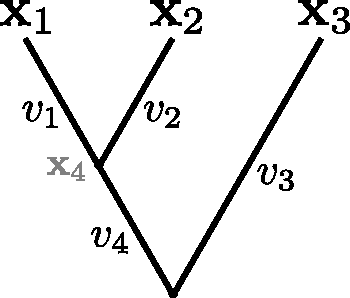
\includegraphics[scale=0.6]{pruning_example_tree_B}
	\caption[Example of phylogeny used to compute the likelihood of a multivariate Brownian-motion model using the new pruning algorithm.]{Example of phylogeny used to compute the likelihood of a multivariate Brownian-motion model using the new pruning algorithm.}
	\label{fig:example_phylo}
\end{figure}

\begin{figure}[h]
	\centering
	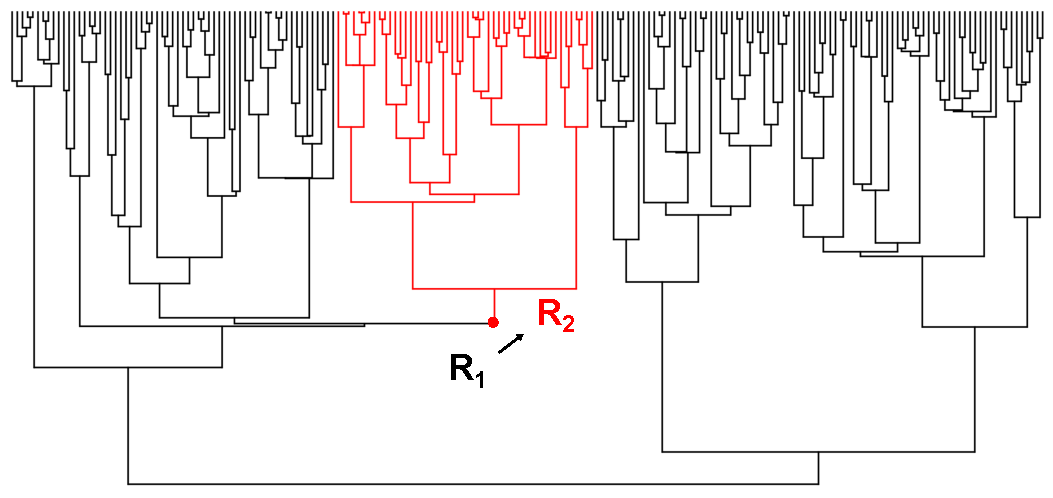
\includegraphics[scale=0.85]{phylogeny_example}
	\caption[Example of phylogeny used for the simulation study.]{Example of phylogeny used for the simulation study. We simulated phylogenies with 200 tips using a homogeneous birth-death model. Then, we randomly selected one node with exact 50 daughter tips to set the location of the transition between the background rate regime $\mathbf{R_{1}}$ and the focus clade regime $\mathbf{R_{2}}$ showed in red.}
	\label{fig:phylogeny_sims}
\end{figure}

\begin{figure}[h]
	\centering
	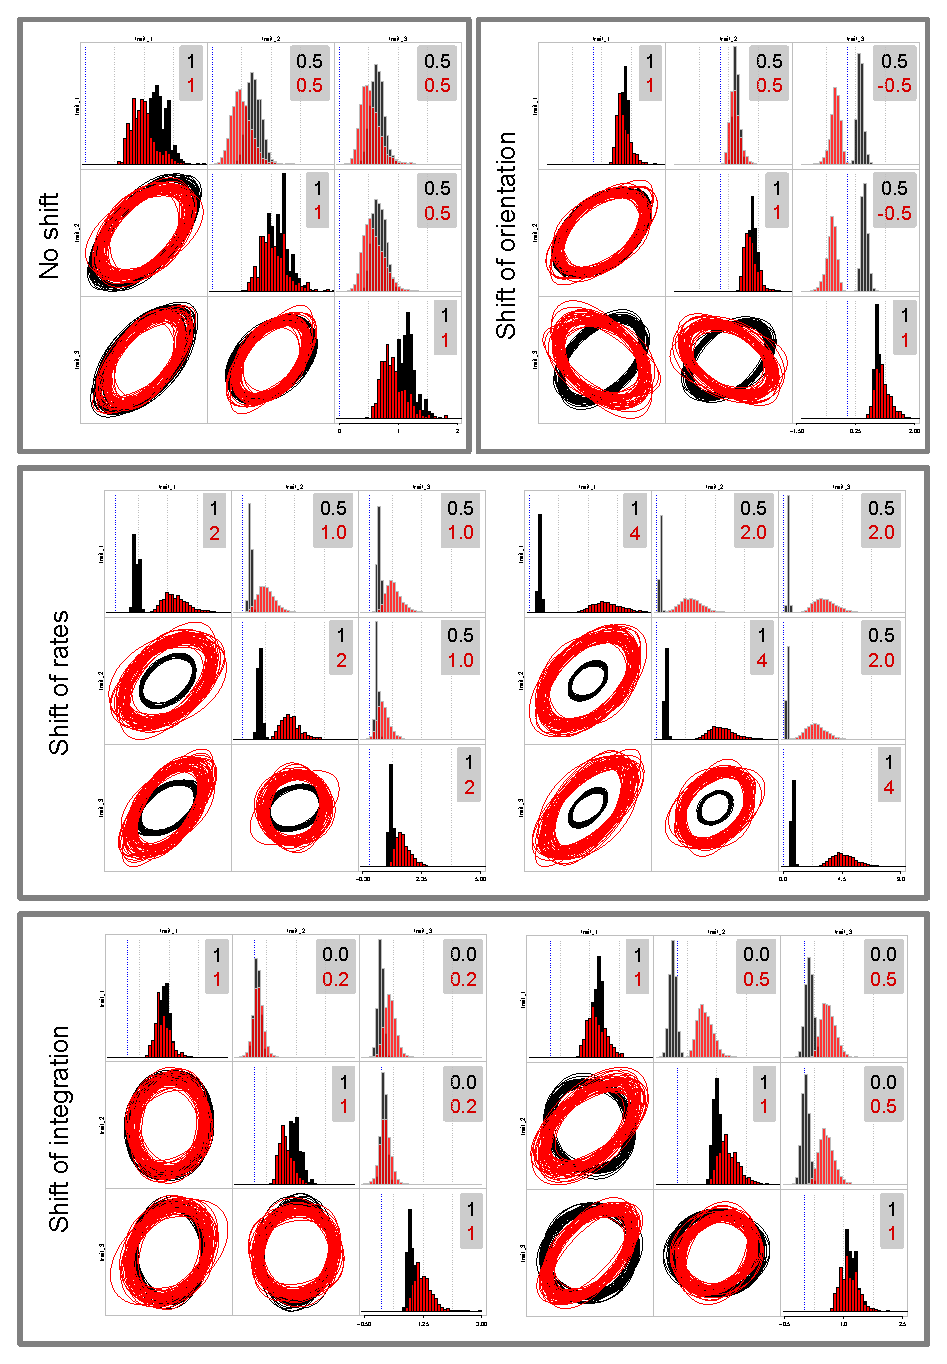
\includegraphics[scale=0.60]{posterior_sims_big_plate}
	\caption[Example of posterior distribution for the six simulation treatments with three traits each.]{Example of posterior distribution for the six simulation treatments with three traits each. Top-left plot shows the results with no shift in the evolutionary rate matrix regime and top-right shows the results with a shift in the orientation of $\mathbf{R}$. Middle row are results with a shift in the rates of evolution of each trait and bottom row shows the results when the strength of the evolutionary correlation shifts between regimes. Estimates for the background regime are showed in black and for the focus regime in red (see Fig. \ref{fig:phylogeny_sims}). For each plot: diagonal histograms show evolutionary rates (variances) for each trait, upper-diagonal histograms show pairwise evolutionary covariation (covariances), and lower-diagonal ellipses are samples from the posterior distribution showing the 95\% confidence interval of each bivariate distribution. Numbers in the top left of histograms are the true value used for each simulation; background rate regimes are showed in black and focus clade regimes in red. Table \ref{tab:model_test} shows the aggregate results for each simulation replicate: `Single' and `Orient' correspond to top-left and top-right plots. `Rates' I and II are middle row left and right plots. `Integ' I and II are bottom row left and right plots. The two replicates in the middle and bottom rows differ in the strength of the shift between regimes, left is weak and right is strong shift.}
	\label{fig:posterior_sims}
\end{figure}

\begin{figure}[h]
	\centering
	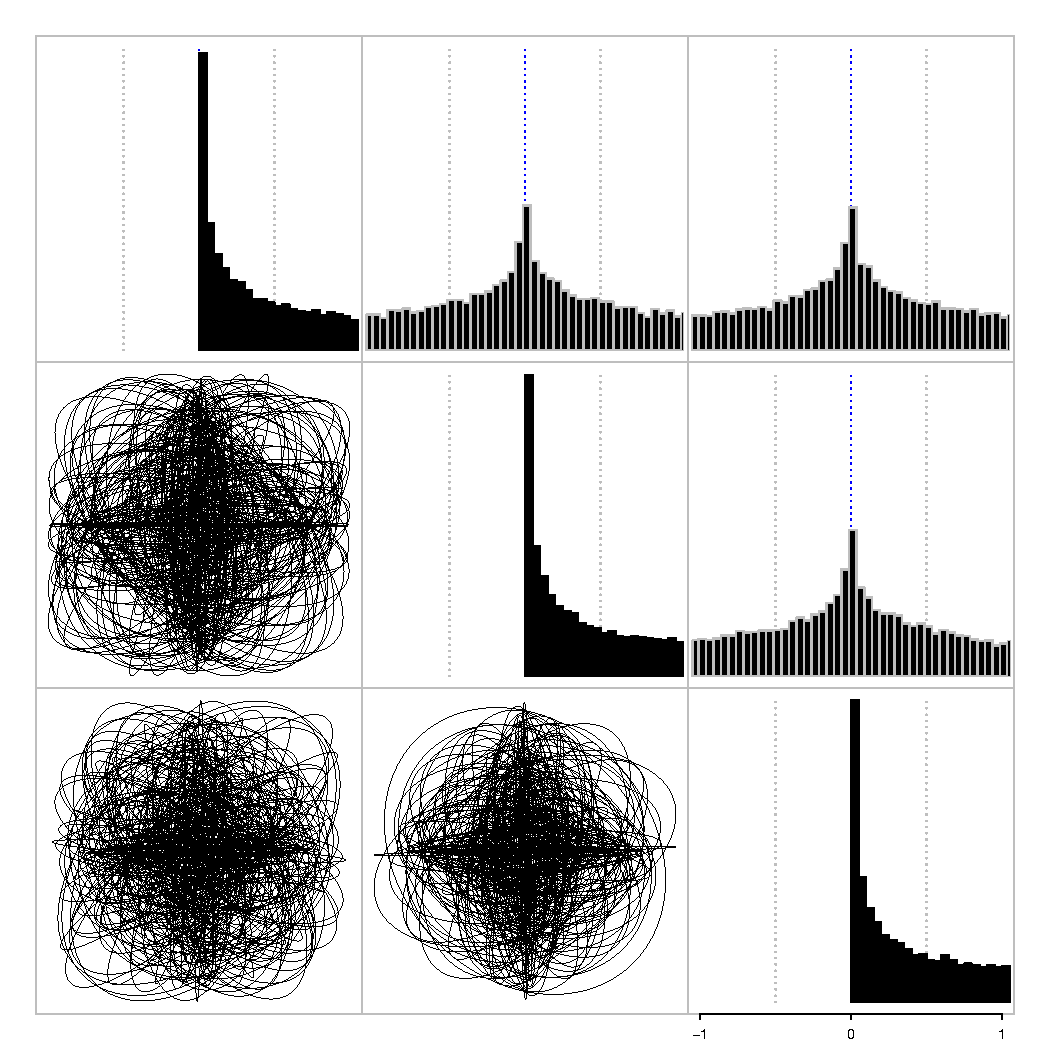
\includegraphics[scale=0.7]{prior_empirical_width_edit}
	\caption[Prior distribution for the evolutionary rate matrix ($\mathbf{R}$) used for all analyses.]{Prior distribution for the evolutionary rate matrix ($\mathbf{R}$) used for all analyses. Plate shows samples in the interval between -1 and 1 from the prior for a model with three traits. Diagonal plots represent the prior for evolutionary rates (variances) for each trait, upper-diagonal plots show pairwise evolutionary covariation (covariances), and lower-diagonal are samples from the posterior distribution of ellipses showing the 95\% confidence interval of each bivariate distribution.}
	\label{fig:prior}
\end{figure}

\begin{figure}[h]
	\centering
	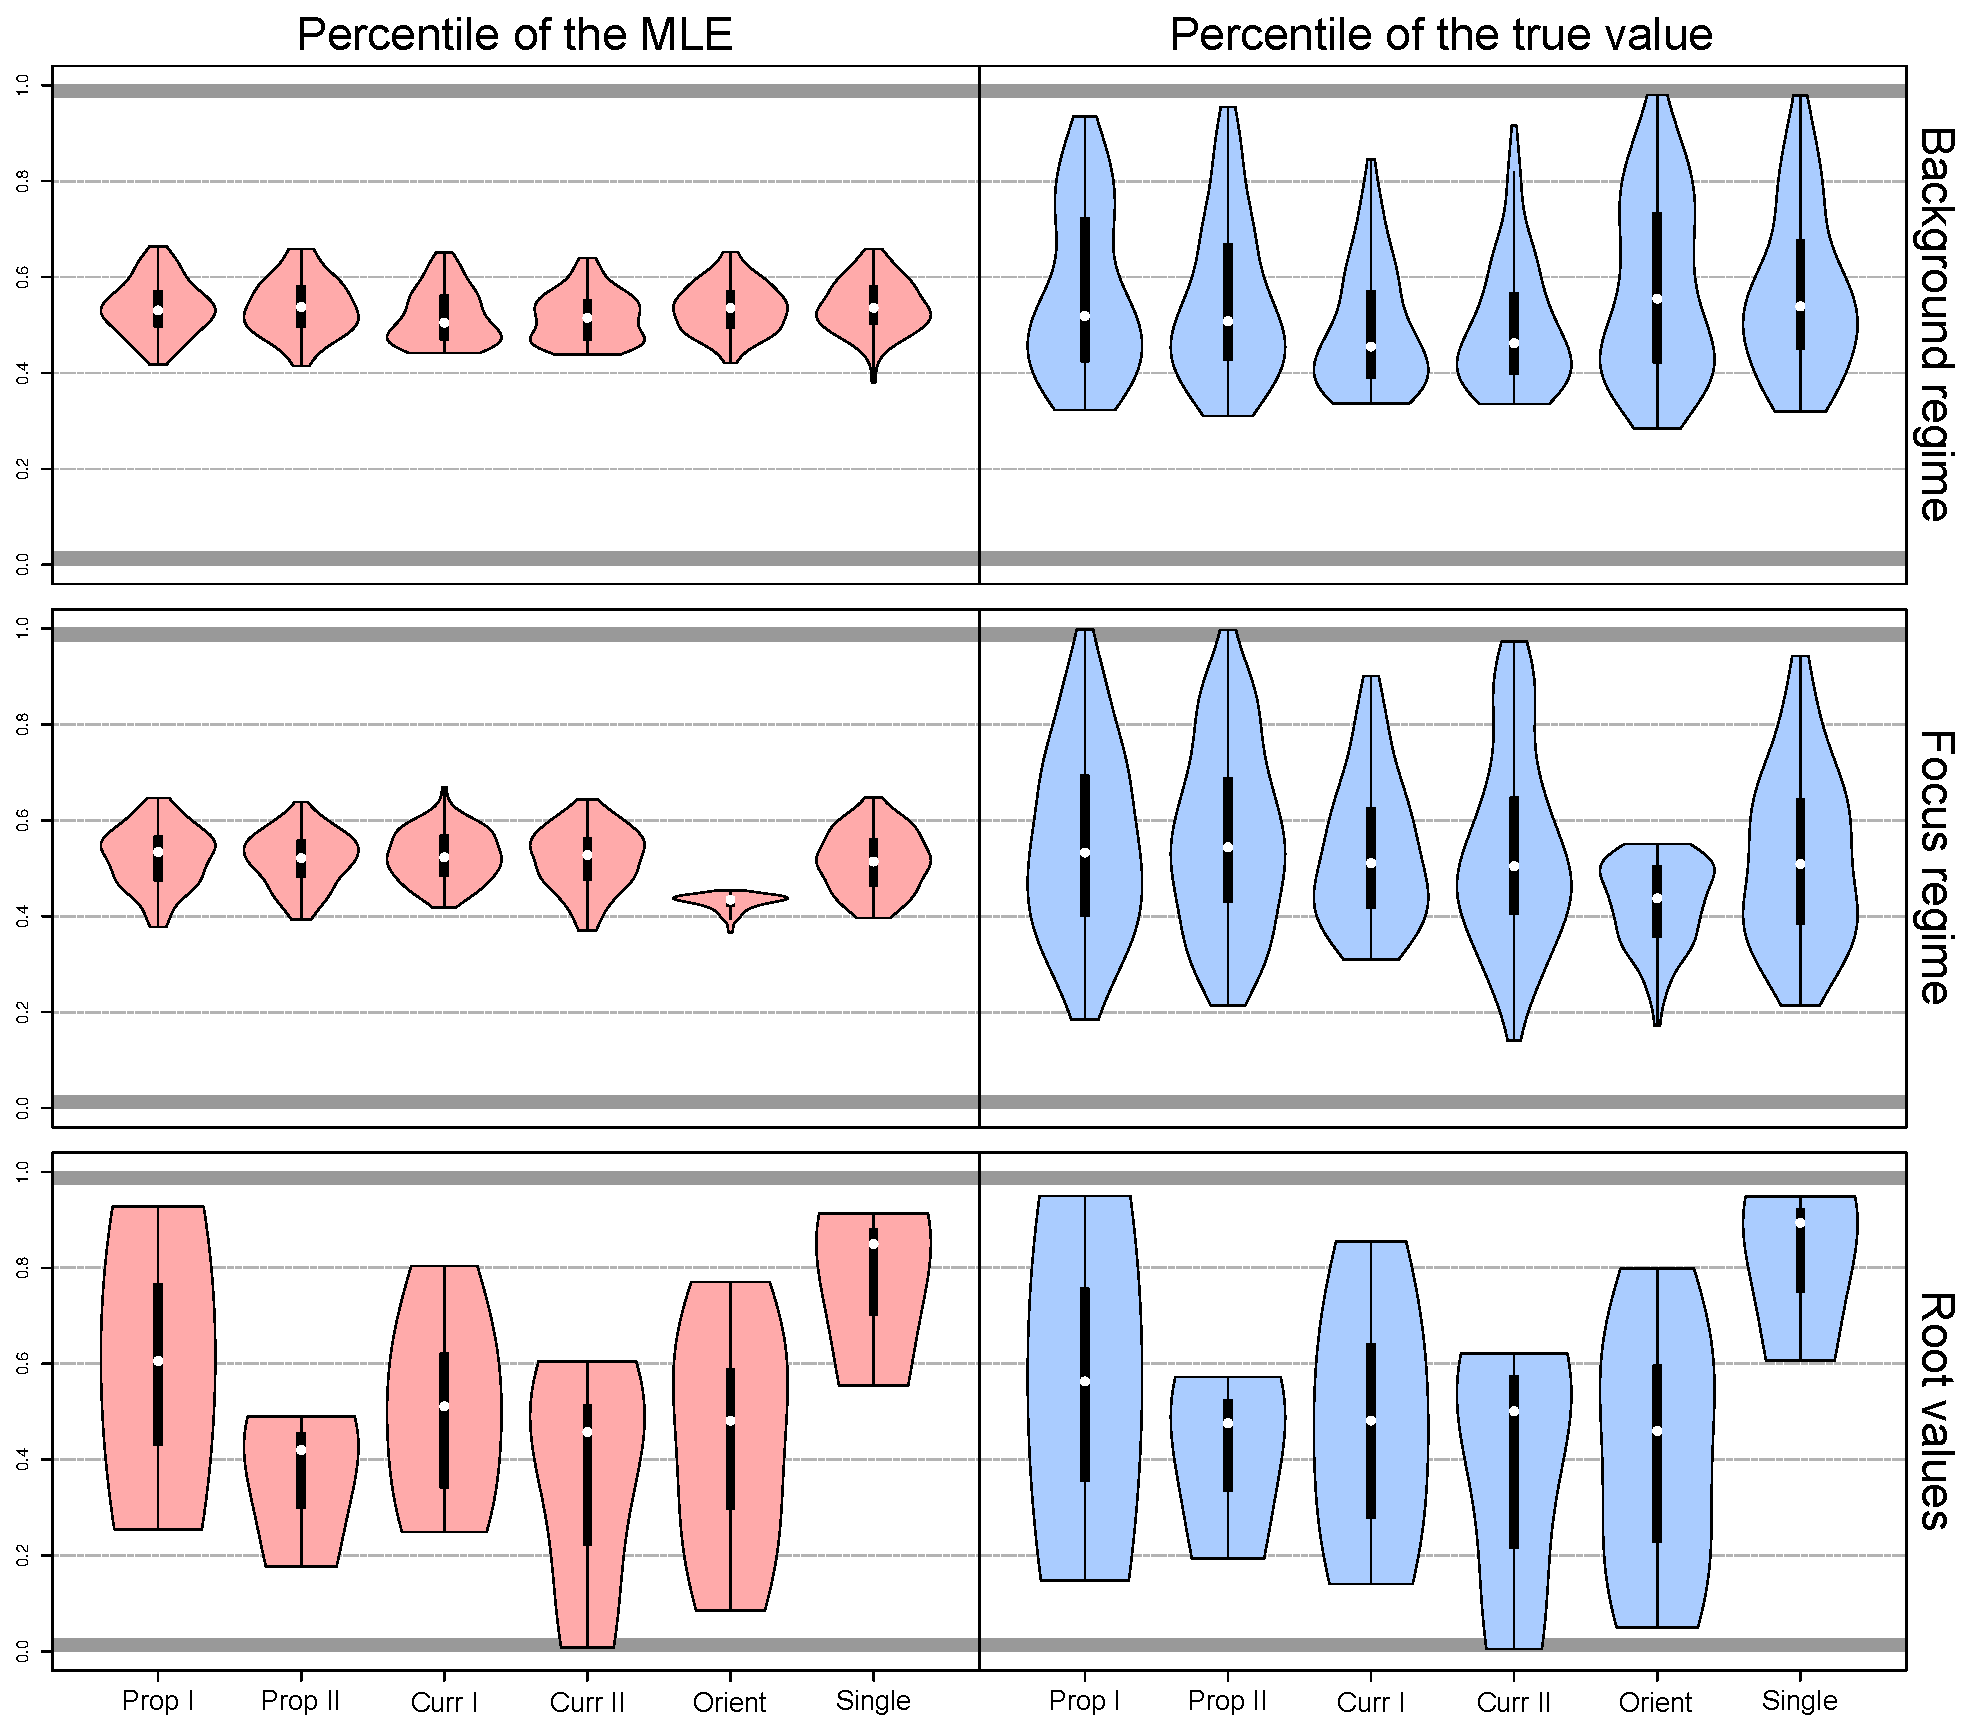
\includegraphics[scale=0.4]{percentiles_mle_true_edit}
	\caption[Distribution of percentiles for the maximum likelihood estimate (MLE) of the full model and for the true value of the simulations with respect to the posterior distribution of each simulation replicate.]{Distribution of percentiles for the maximum likelihood estimate (MLE) of the full model and for the true value of the simulations with respect to the posterior distribution of each simulation replicate. Plots to the left (pink) show the percentiles for the MLE whereas plots to the right (blue) show the percentiles for the true value of the simulations. Most of the density across all simulation scenarios and parameters is within the 95\% HPD of the posterior distribution.}
	\label{fig:quantiles}
\end{figure}

\begin{figure}[h]
	\centering
	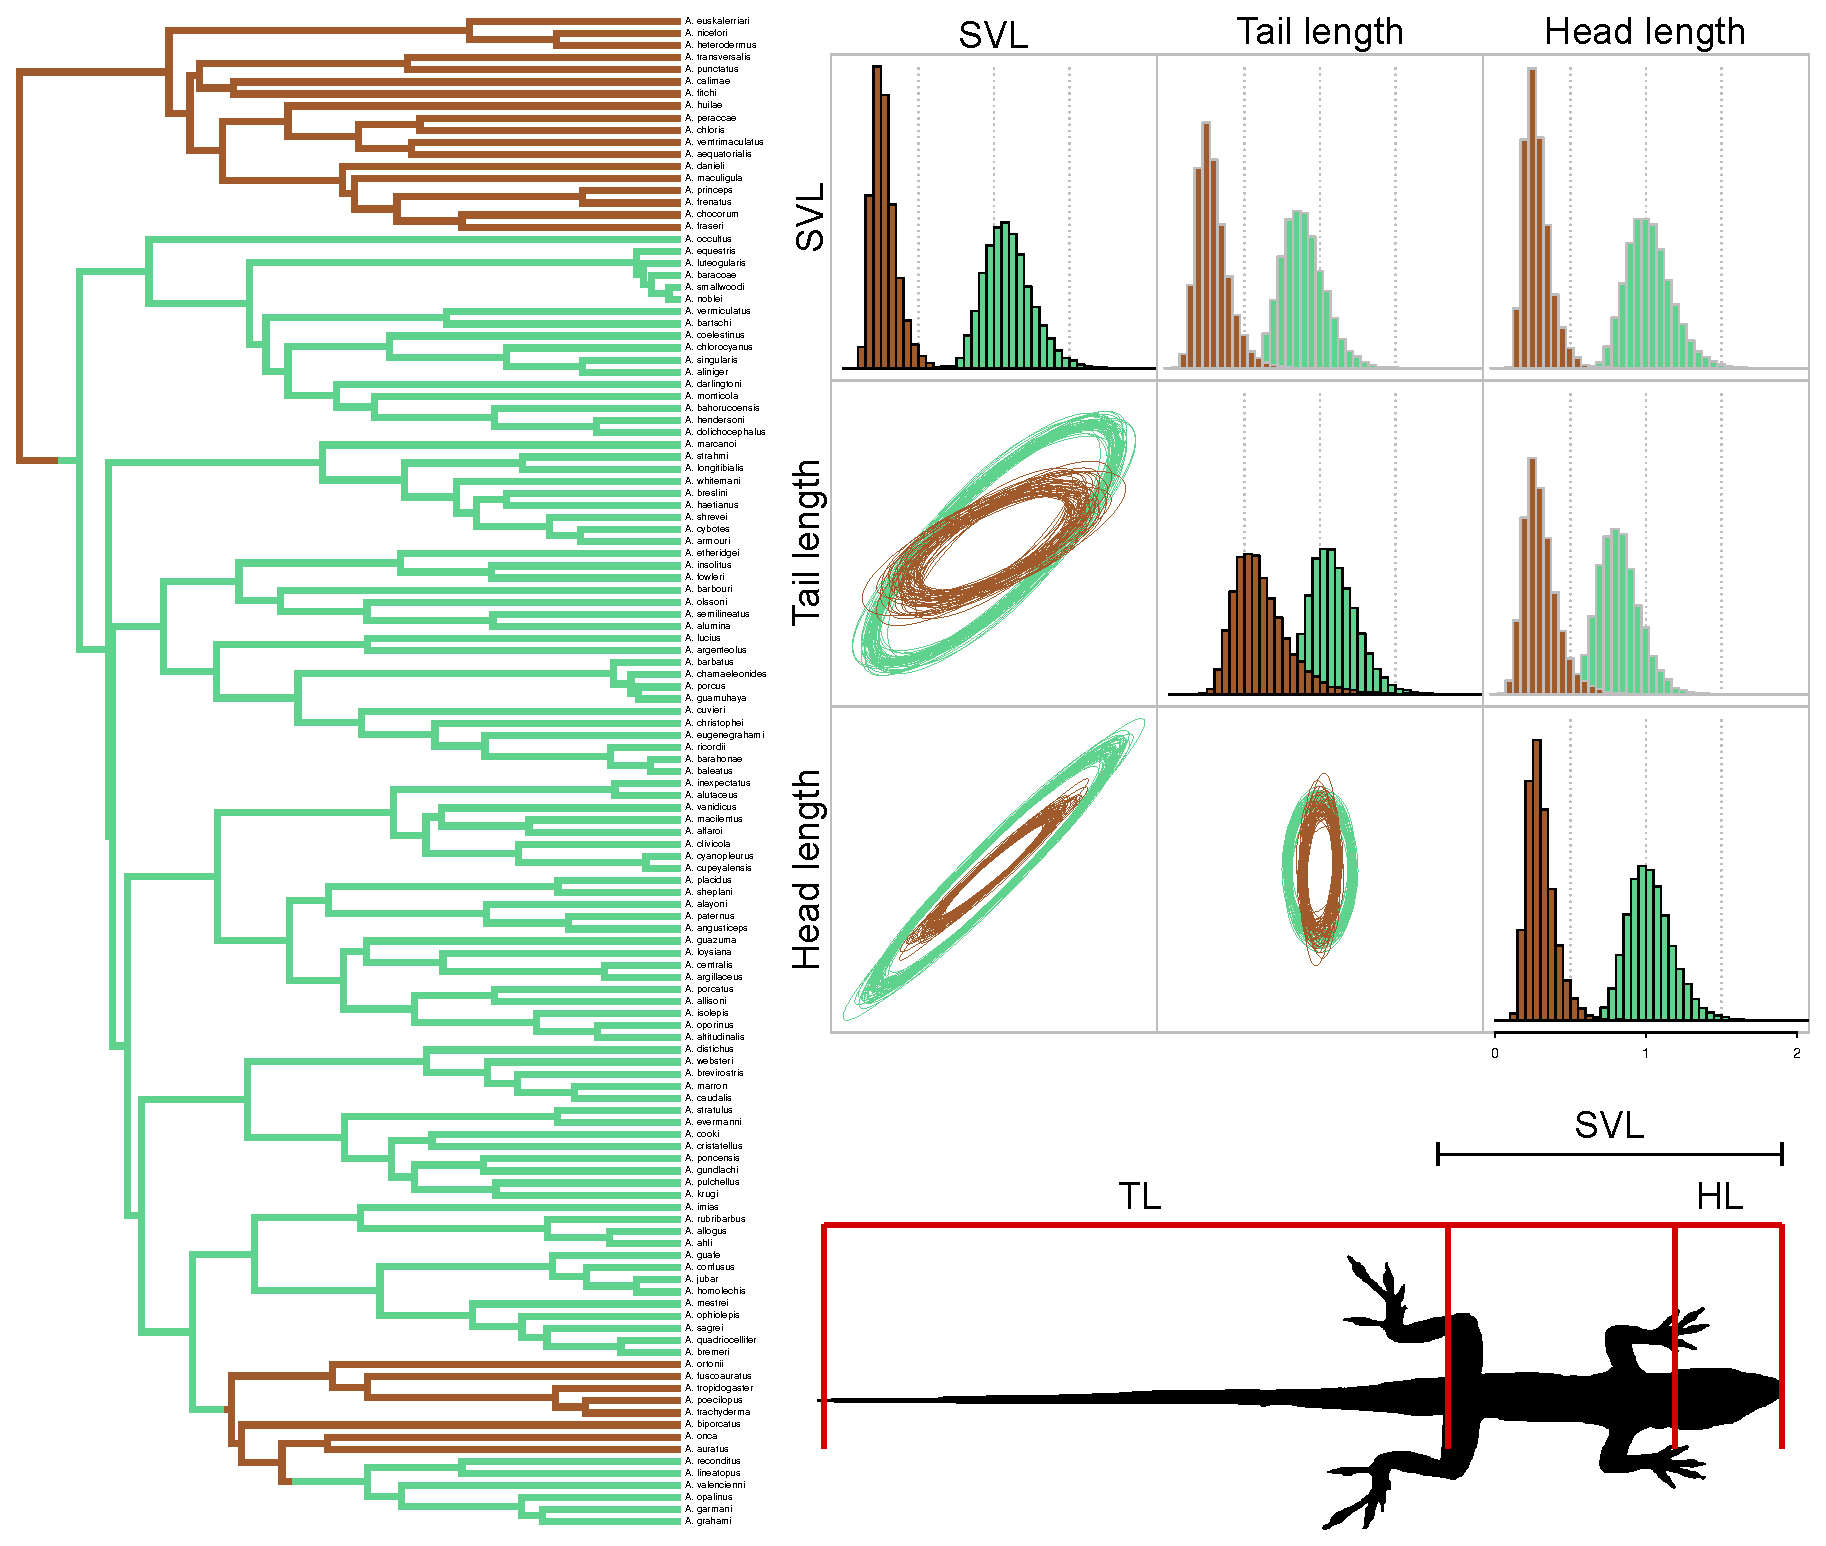
\includegraphics[scale=0.5]{anoles_figure}
	\caption[Posterior distribution of the $\mathbf{R}$ matrix regimes fitted to the island anole (green) and mainland anole (brown) lineages.]{Posterior distribution of the $\mathbf{R}$ matrix regimes fitted to the island anole (green) and mainland anole (brown) lineages. Left figure shows the maximum clade credibility tree (MCC) from \citet{gamble_anolis_2014} with only the taxa used in this study. State reconstruction for the branches was performed with a stochastic map simulation using `mainland' as the root state for the genus. Right upper plot shows the posterior distribution of parameter estimates for the evolutionary rate matrices. Diagonal plots show evolutionary rates (variances) for each trait, upper-diagonal plots show pairwise evolutionary covariation (covariances), and lower-diagonal are samples from the posterior distribution of ellipses showing the 95\% confidence interval of each bivariate distribution. Right bottom figure shows a representation of each trait (TL: tail length; HL: head length; SVL: snout-vent length).}
	\label{fig:anoles}
\end{figure}

\begin{figure}[h]
	\centering
	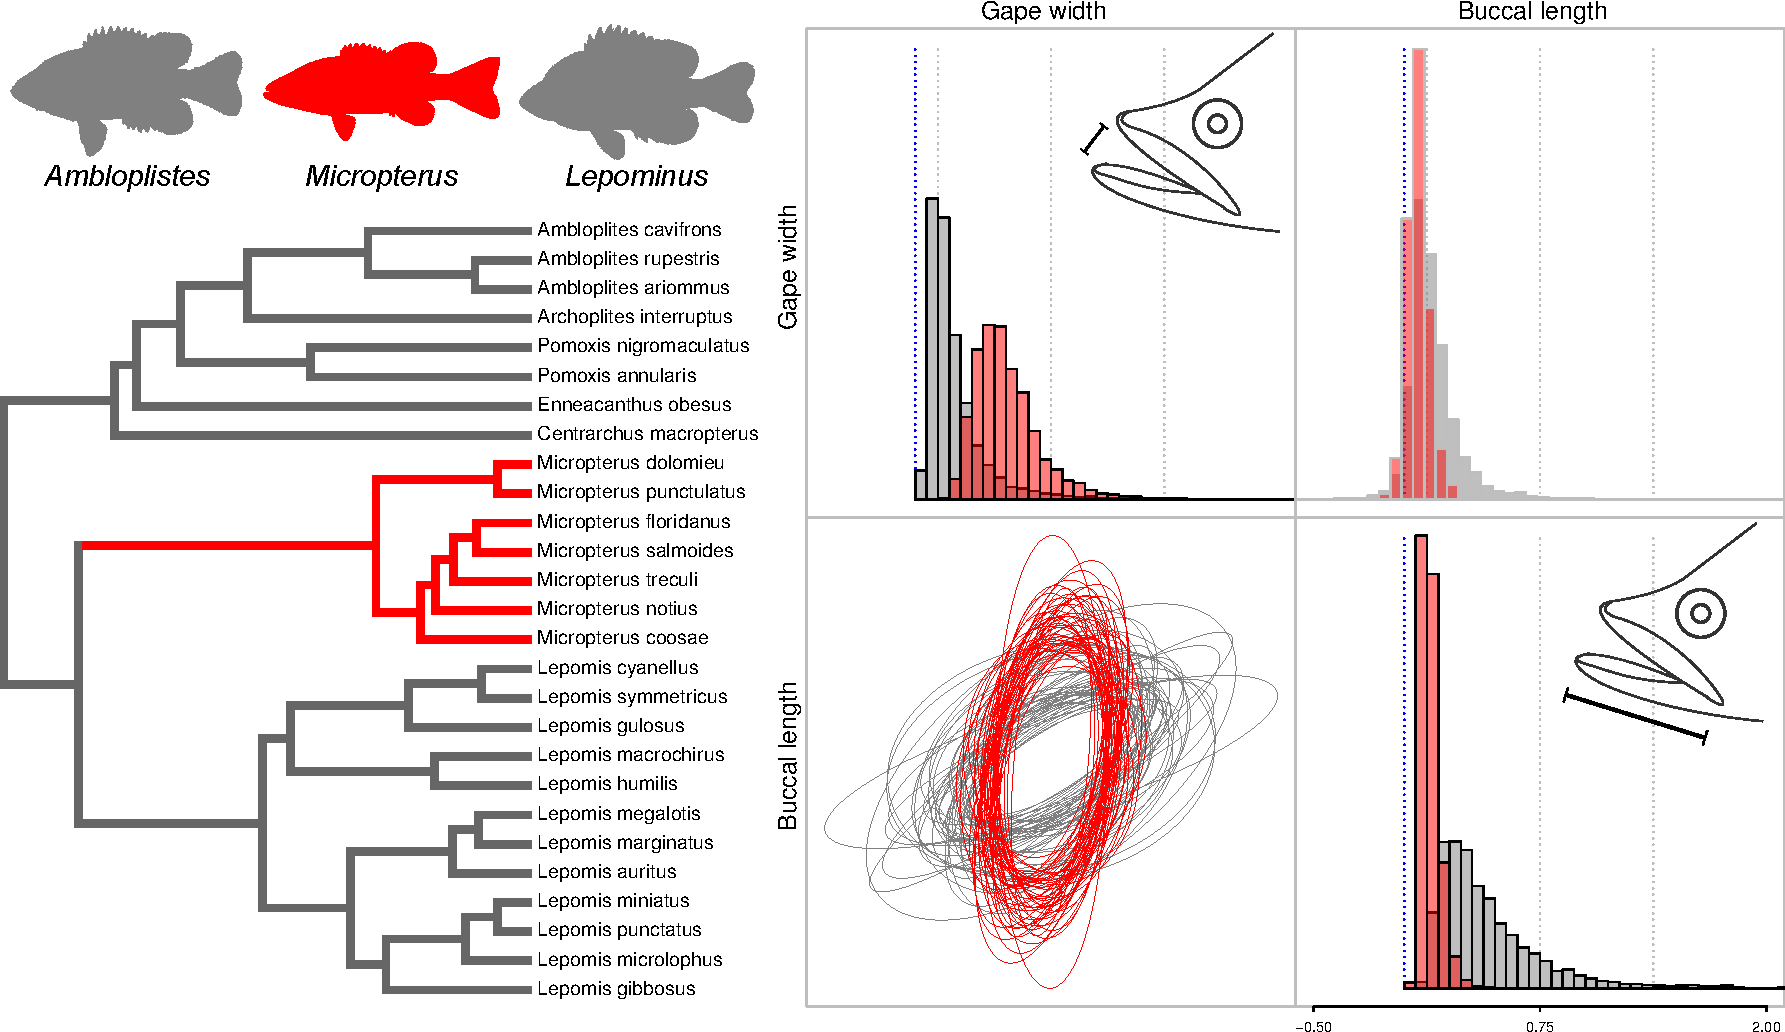
\includegraphics[scale=0.5]{results_centrarchidae}
	\caption[Posterior distribution of the $\mathbf{R}$ matrix regimes fitted to the background group and to the \textit{Micropterus} clade.]{Posterior distribution of the $\mathbf{R}$ matrix regimes fitted to the background group (gray) and to the \textit{Micropterus} clade (red). Left figure shows the phylogeny from \citep{revell_phylogenetic_2009} and the silhouette of some representatives of the Centrarchidae genera. Right plot shows the posterior distribution of parameter estimates for the evolutionary rate matrices. Diagonal plots show evolutionary rates (variances) for each trait, upper-diagonal plots show pairwise evolutionary covariation (covariances), and lower-diagonal are samples from the posterior distribution of ellipses showing the 95\% confidence interval of each bivariate distribution.}
	\label{fig:centrarchidae}
\end{figure}

\begin{figure}[h]
	\centering
	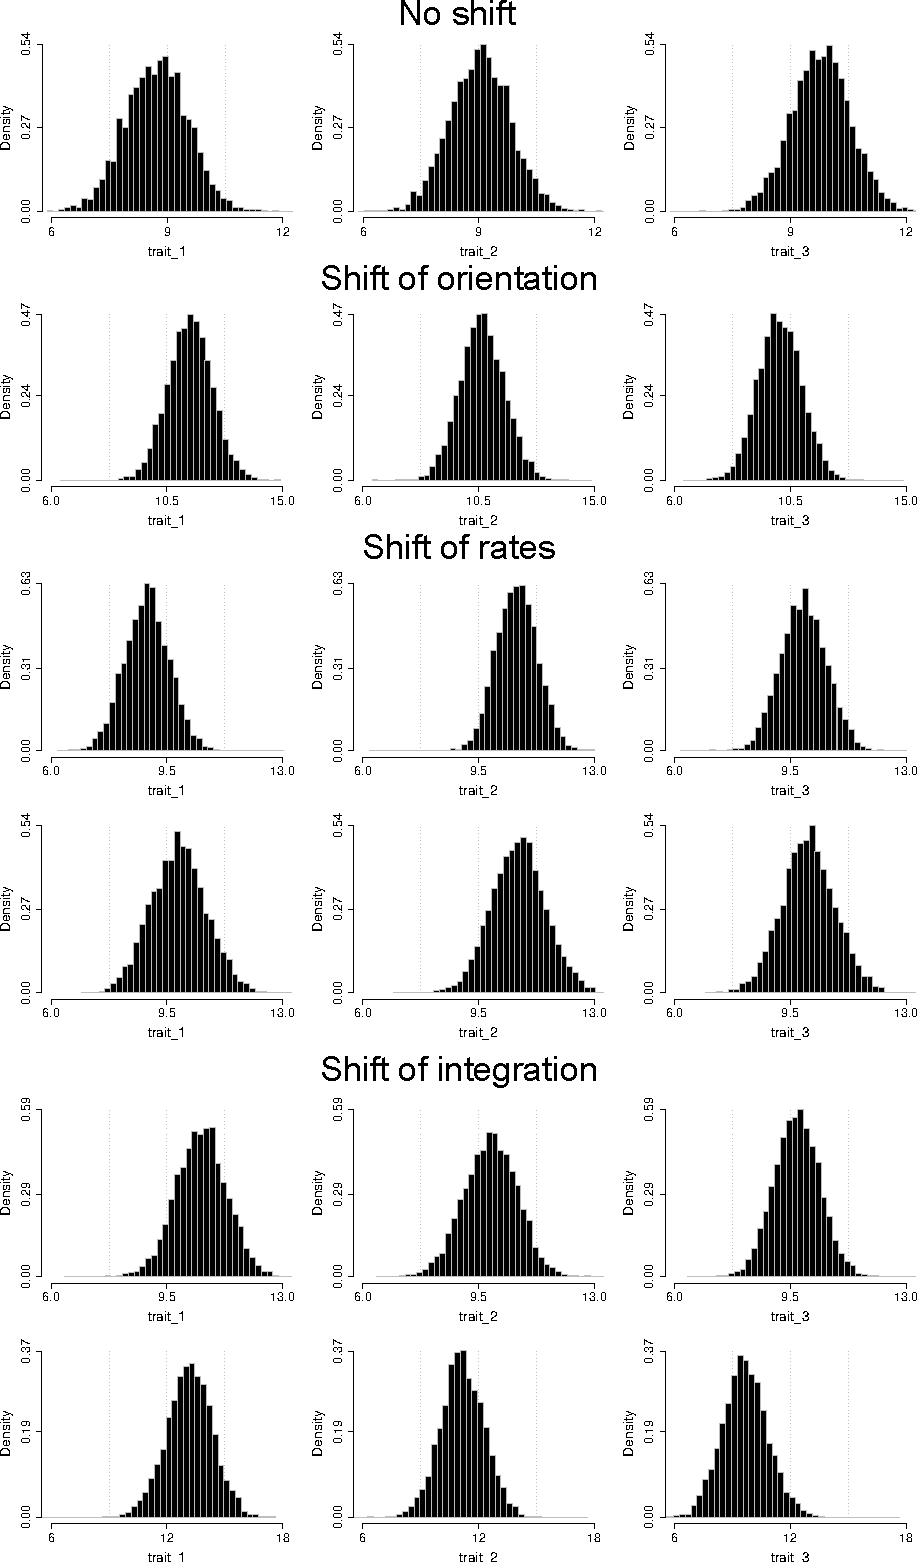
\includegraphics[scale=0.6]{root_sims_plate}
	\caption[Example of posterior distribution of root values for the six simulation treatments with three traits each.]{Example of posterior distribution of root values for the six simulation treatments with three traits each. Simulation treatments are the same as showed on Figure \ref{fig:posterior_sims}. Top and bottom plots for `Shift of rates' and `Shift of integration' treatments correspond to the left and right plots of the same treatments on Figure \ref{fig:posterior_sims}, respectively. The true value for the ancestral state of each trait in all simulations was equal to 10.}
	\label{fig:sup_root_sims}
\end{figure}

\begin{figure}[h]
	\centering
	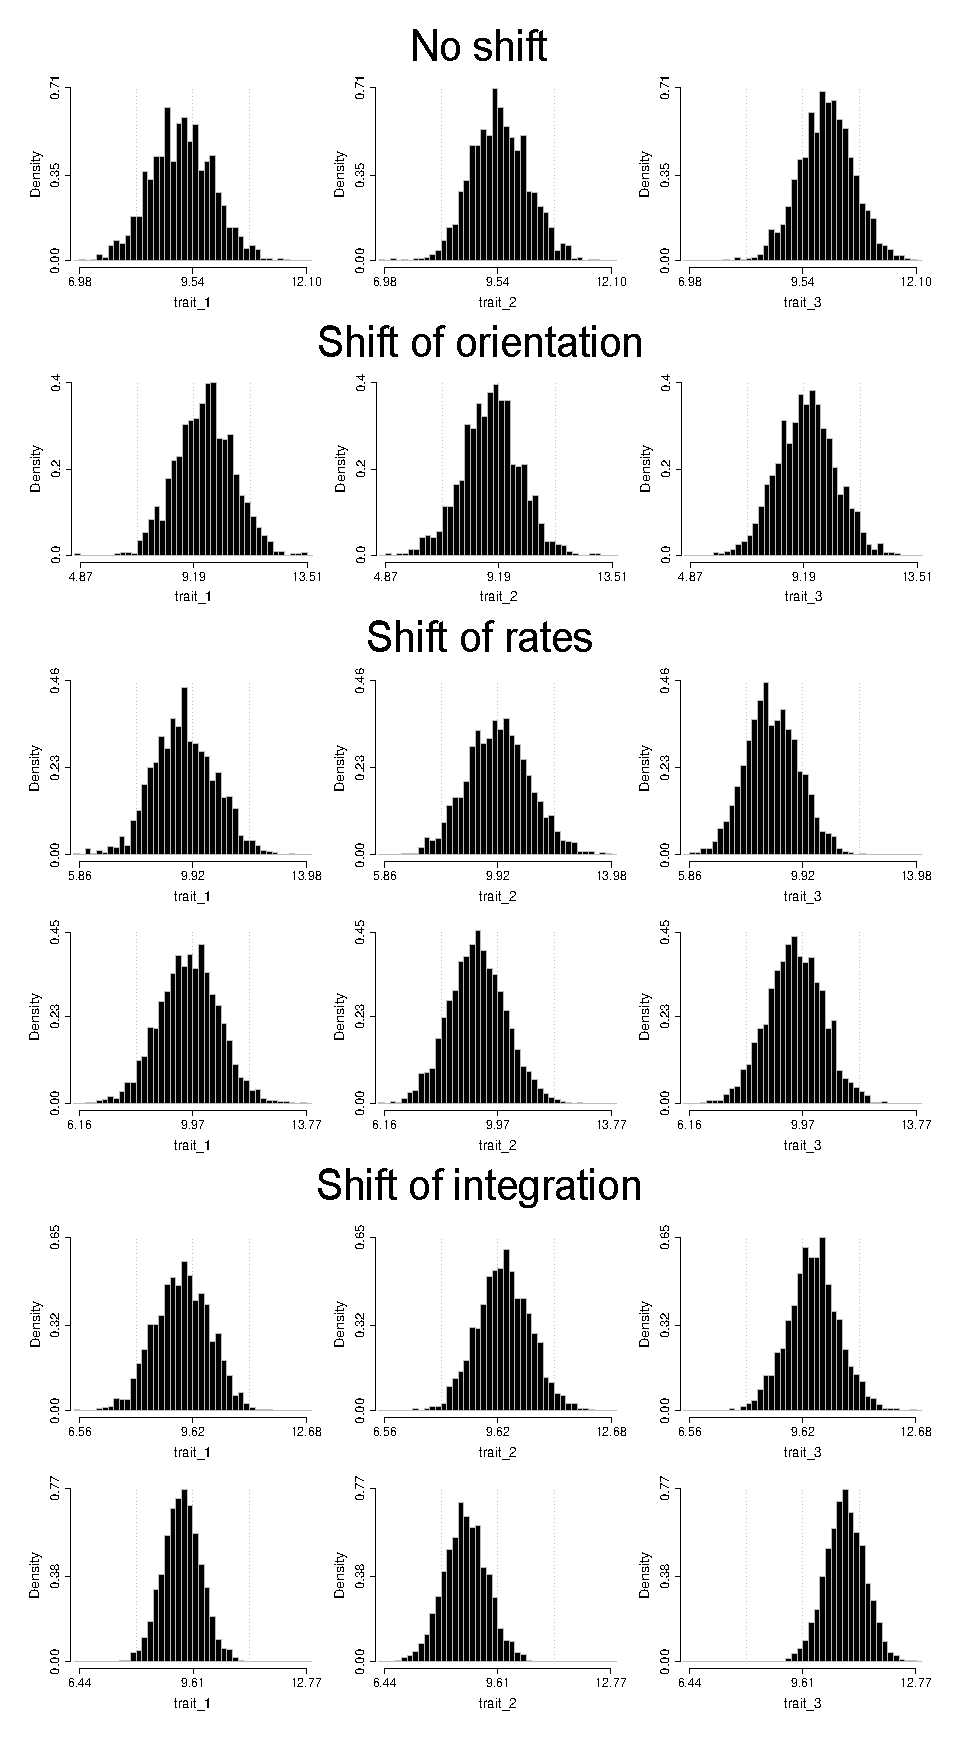
\includegraphics[scale=0.6]{plate_root_value_flat}
	\caption[Example of posterior distribution of root values for the six simulation treatments with three traits each using a uniform prior for the vector of root values.]{Example of posterior distribution of root values for the six simulation treatments with three traits each using a uniform prior for the vector of root values. Simulation treatments are the same as showed on Figure \ref{fig:posterior_sims} and Figure \ref{fig:sup_root_sims}. The true value for the ancestral state of each trait in all simulations was equal to 10.}
	\label{fig:sup_root_sims_flat}
\end{figure}

\begin{figure}[h]
	\centering
	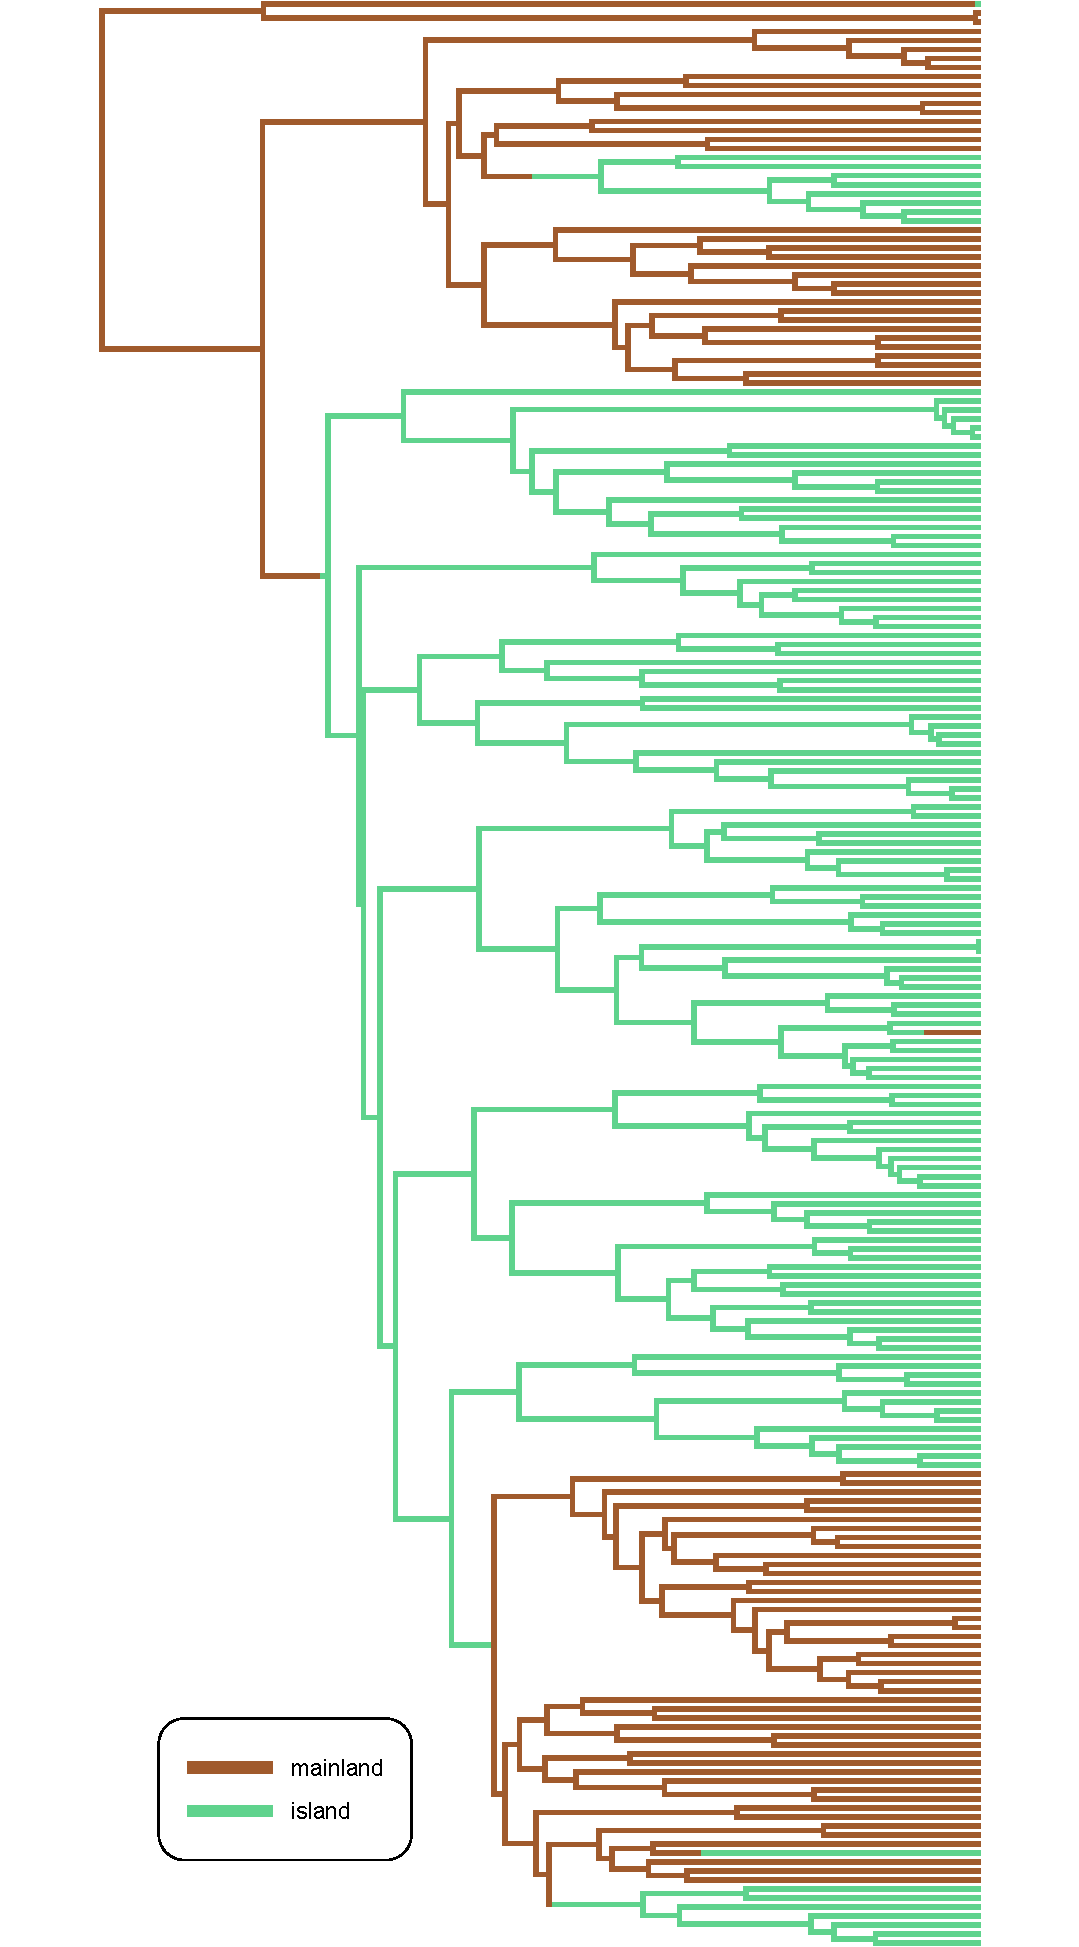
\includegraphics[scale=0.5]{Gamble_full_biogeo}
	\caption[Maximum clade credibility tree from \citet{gamble_anolis_2014} study showing the distribution of `mainland' and `island' anole species.]{Maximum clade credibility tree from \citet{gamble_anolis_2014} study showing the distribution of `mainland' and `island' anole species. The species `sp\_nov\_1', `sp\_nov\_2', and `sp\_nov\_3'  were excluded from the phylogenetic tree. Data for the distribution of anole species and outgroups were compiled from \citet{nicholson_mainland_2005}, \citet{losos_lizards_2009}, \citet{thomas_body_2009}, Reptile database (reptile-database.org) and GBIF (gbif.org). Ancestral state reconstruction was performed using stochastic mapping with the `all rates different' model and the root state set as `mainland' \citep{nicholson_mainland_2005, losos_lizards_2009}. }
	\label{fig:biogeo_gamble}
\end{figure}

\begin{figure}[h]
	\centering
	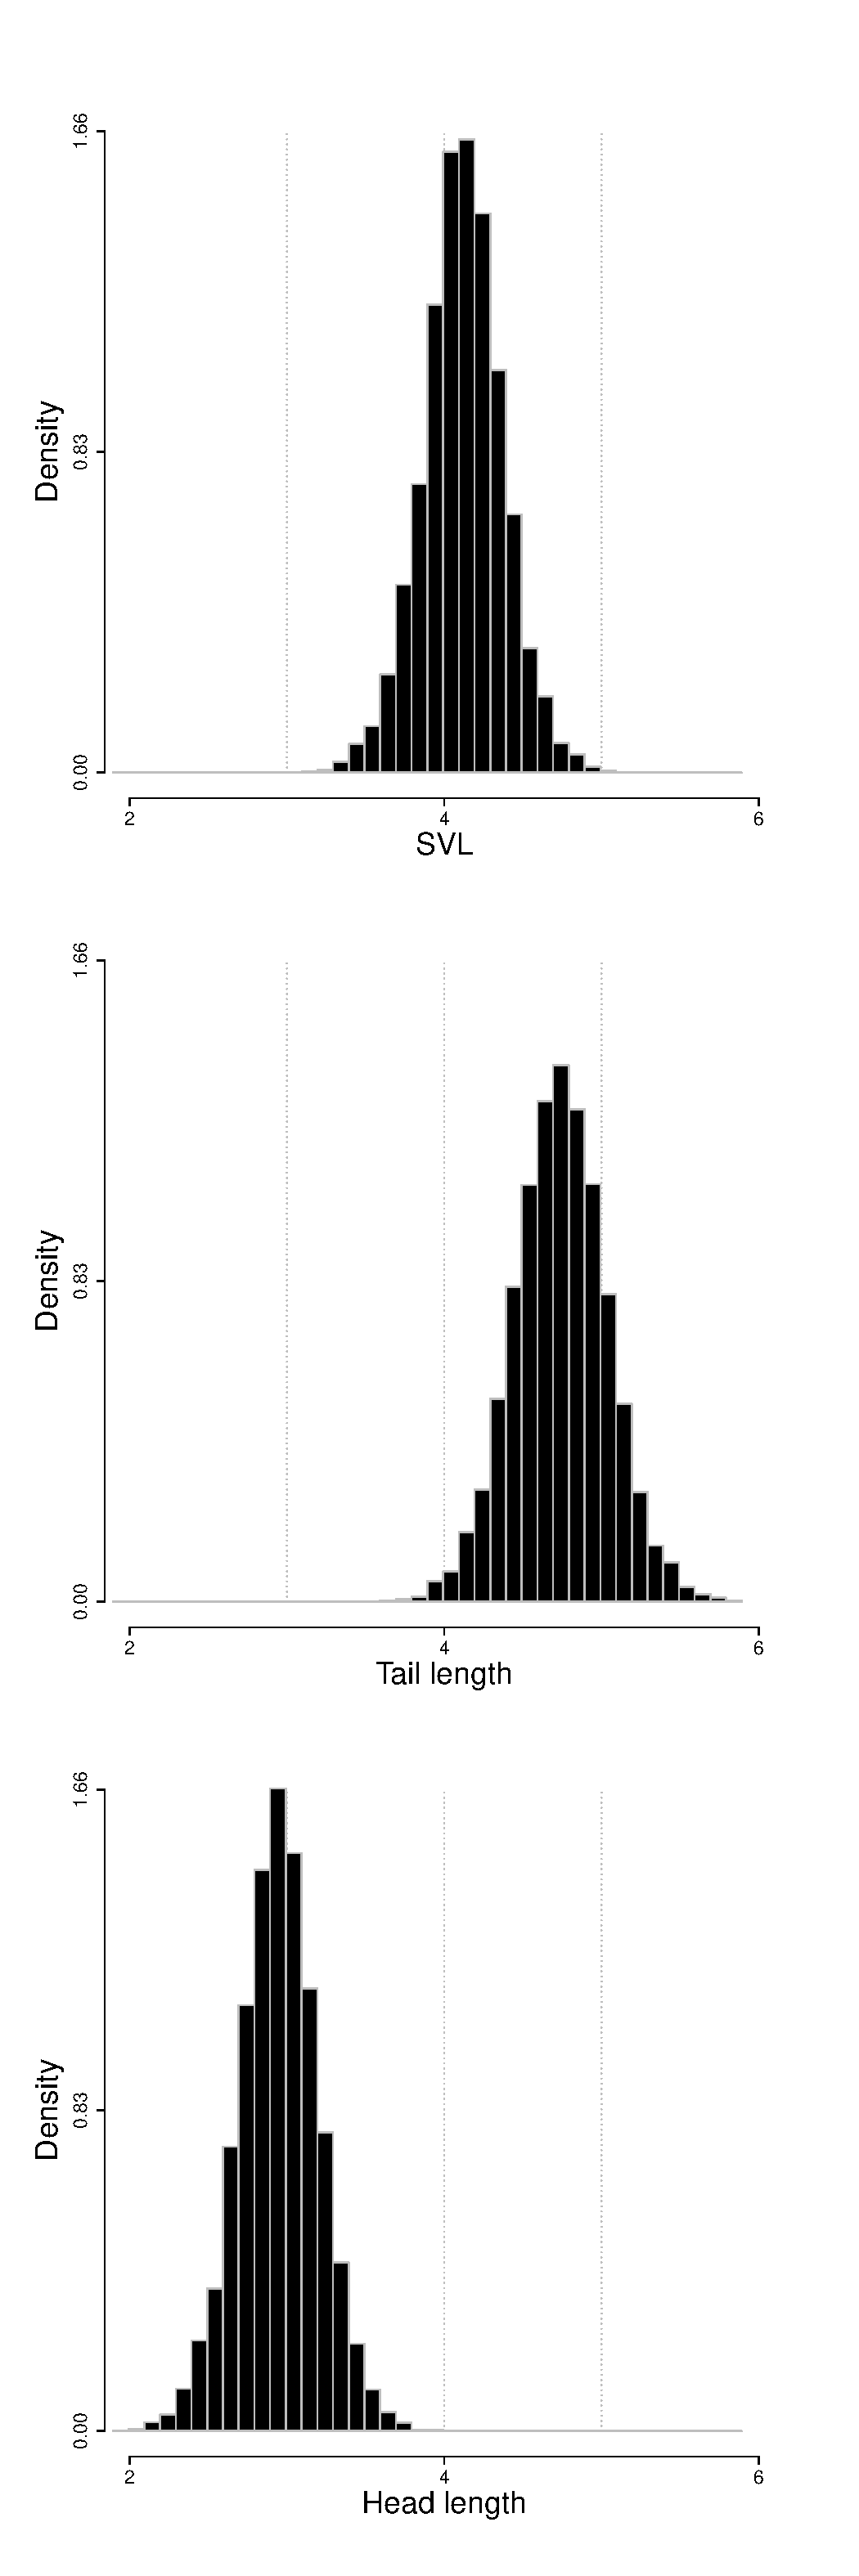
\includegraphics[scale=0.3]{anoles_root_plot}
	\caption[Posterior distribution of root values fitted to the island and mainland anole lineages.]{Posterior distribution of root values fitted to the island and mainland anole lineages (SVL: snout-vent length).}
	\label{fig:sup_root_anoles}
\end{figure}

\begin{figure}[h]
	\centering
	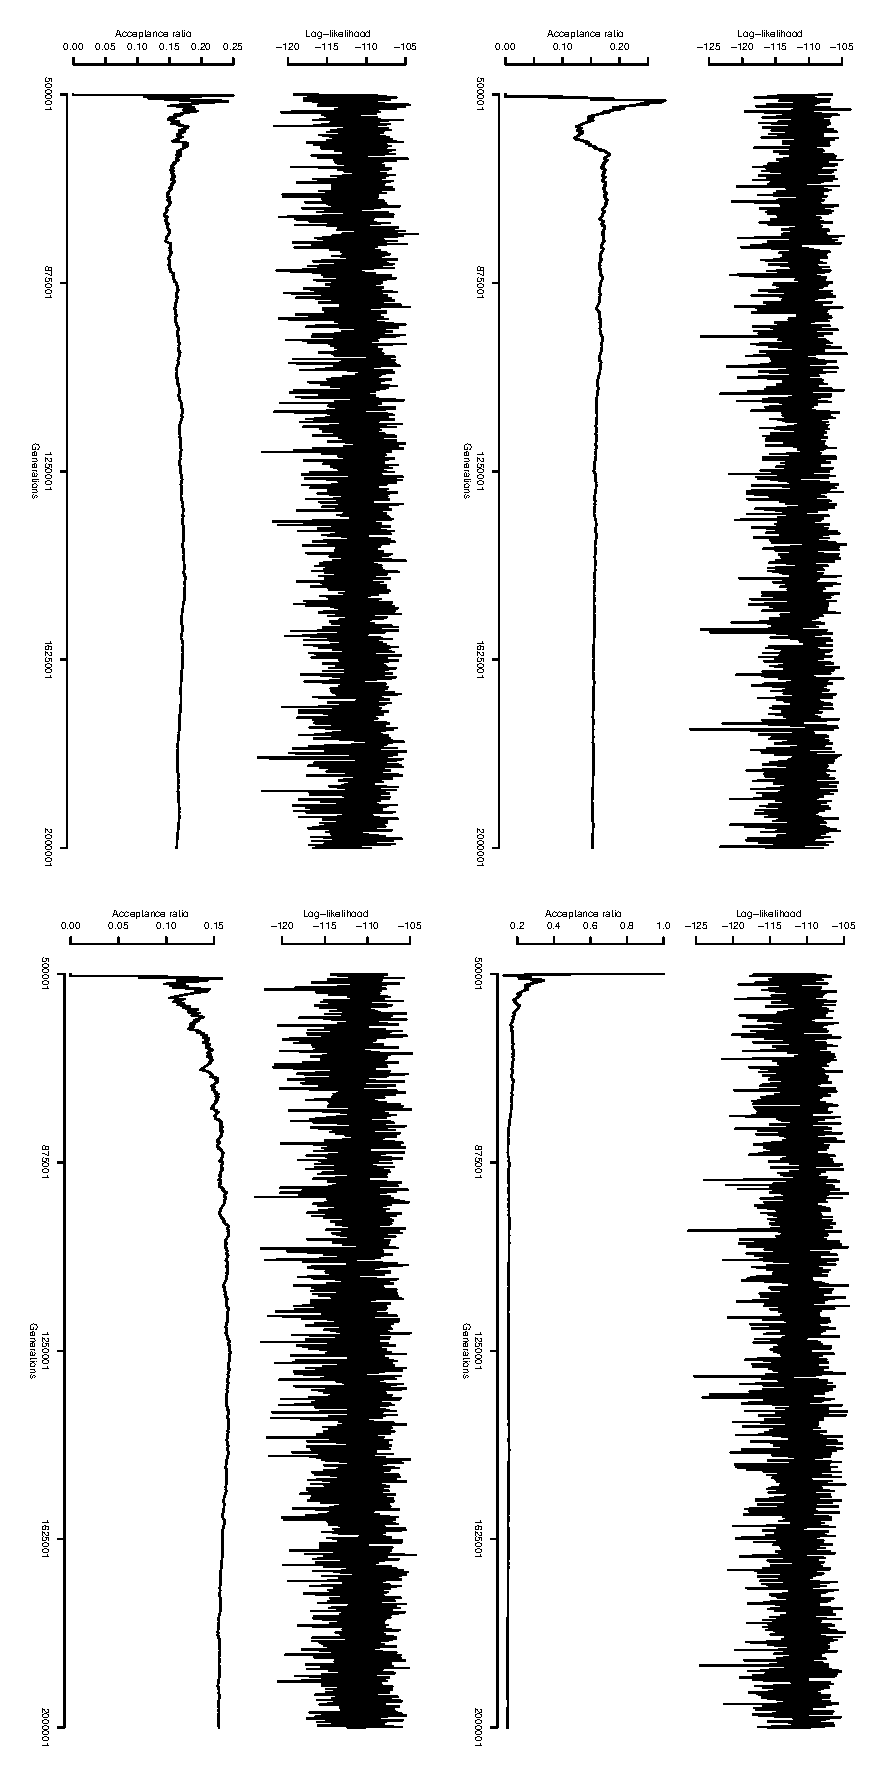
\includegraphics[scale=0.6]{anoles_log_trace_plots}
	\caption[Trace plots of the log-likelihood and the acceptance ratio for the four independent MCMC chains of the island and mainland anole analysis.]{Trace plots of the log-likelihood and the acceptance ratio for the four independent MCMC chains of the island and mainland anole analysis. }
	\label{fig:sup_trace_anoles}
\end{figure}

\begin{figure}[h]
	\centering
	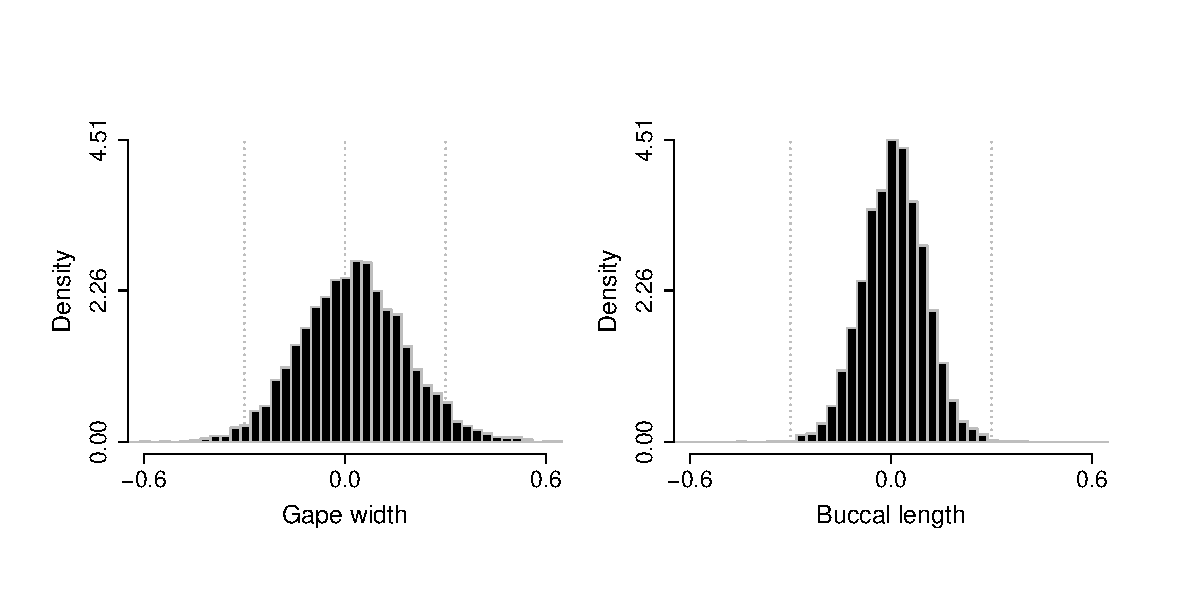
\includegraphics[scale=0.7]{root_plot_centrarchidae}
	\caption[Posterior distribution of root values fitted to the Centrarchidae fishes.]{Posterior distribution of root values fitted to the Centrarchidae fishes.}
	\label{fig:sup_root_centrarchidae}
\end{figure}

\begin{figure}[h]
	\centering
	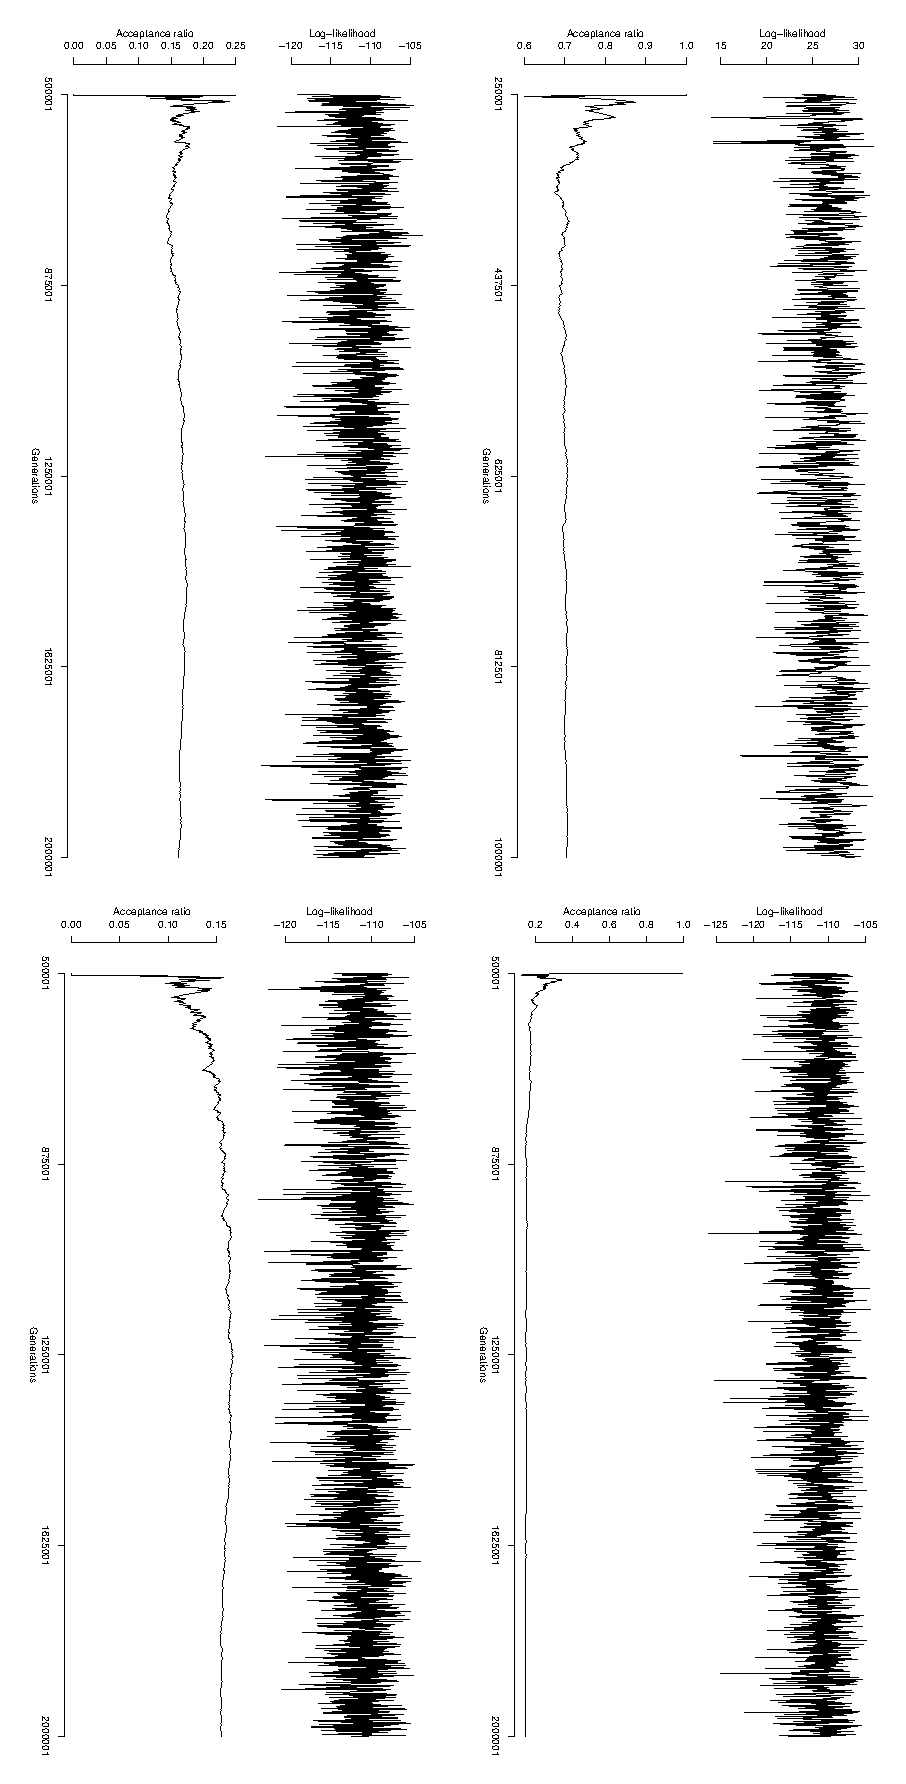
\includegraphics[scale=0.6]{trace_plots_centrarchidae}
	\caption[Trace plots of the log-likelihood and the acceptance ratio for the four independent MCMC chains of the Centrarchidae fishes analysis.]{Trace plots of the log-likelihood and the acceptance ratio for the four independent MCMC chains of the Centrarchidae fishes analysis. }
	\label{fig:sup_trace_centrarchidae}
\end{figure}

\begin{figure}[h]
	\centering
	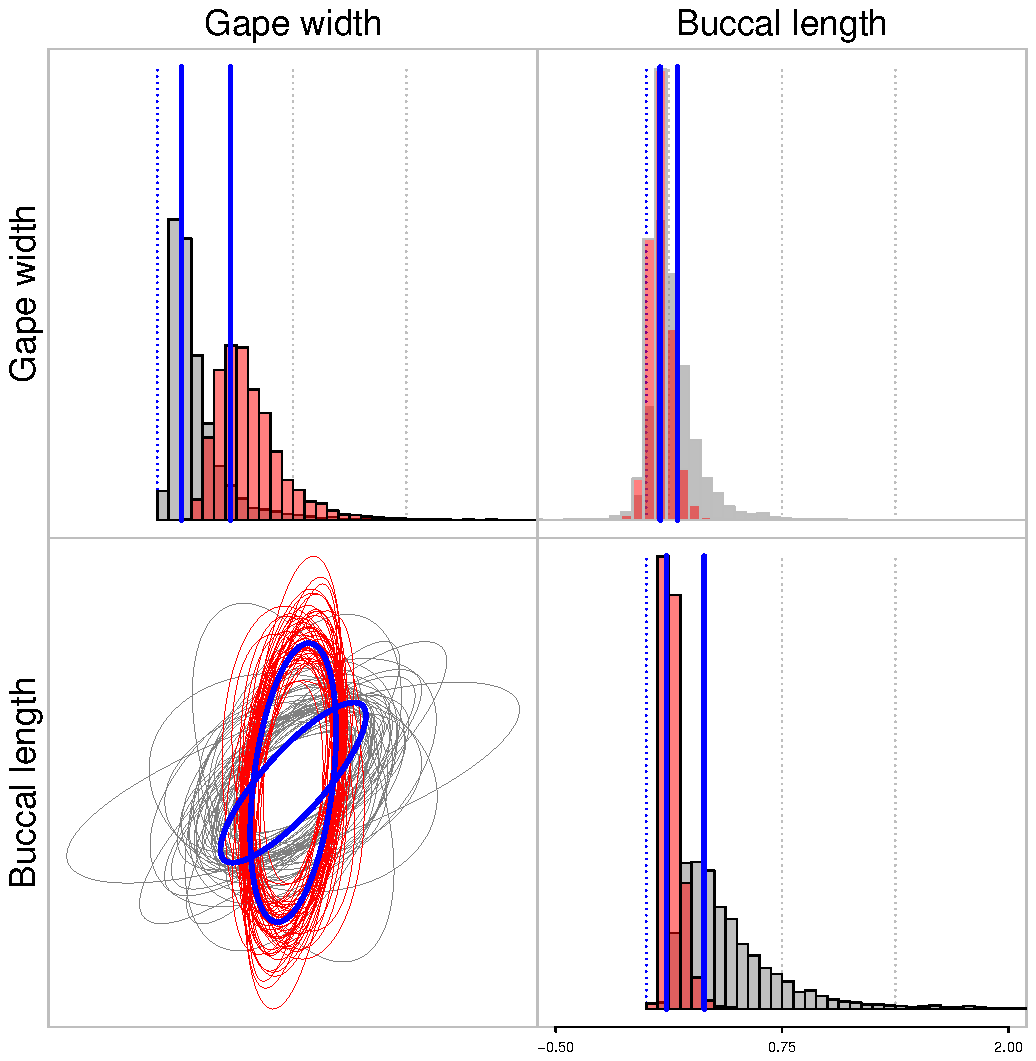
\includegraphics[scale=0.6]{centrarchidae_compare_with_mle}
	\caption[Posterior distribution of the $\mathbf{R}$ matrix regimes fitted to the background group and to the \textit{Micropterus} clade.]{Posterior distribution of the $\mathbf{R}$ matrix regimes fitted to the background group (gray) and to the \textit{Micropterus} clade (red). Maximum likelihood estimate for the same data and phylogenetic tree showed in blue lines. Plot shows the posterior distribution of parameter estimates for the evolutionary rate matrices. Diagonal plots show evolutionary rates (variances) for each trait, upper-diagonal plot show pairwise evolutionary covariation (covariances), and lower-diagonal plot shows samples from the posterior distribution of ellipses showing the 95\% confidence interval of each bivariate distribution.}
	\label{fig:centrarchidae_mle}
\end{figure}

%% The references for ALL chapters will be at the end of the chapters. The references need to come BEFORE any appendices.
\bibliographystyle{sysbio}
\addcontentsline{toc}{chapter}{Bibliography}
\bibliography{GeoMorpho}

%% Appendices would come here:
% \include{Appendices}

\end{document}